\documentclass[parskip=full]{scrartcl}

\usepackage[utf8]{inputenc}			% Umlaute, Sonderzeichen
\usepackage[ngerman]{babel}			% deutsche Sprache
%\usepackage[tocfullflat]{tocstyle}		% Inhaltsverzeichnis
\usepackage{enumitem}				% Listen
\usepackage{graphicx}					% Grafiken
\usepackage{hyperref}					% Hyperlinks
\usepackage[nonumberlist]{glossaries}		% Glossar
\usepackage{amsmath}

% Hurenkinder und Schusterjungen verhindern
\clubpenalty10000
\widowpenalty10000
\displaywidowpenalty=10000

\DeclareRobustCommand{\glossfirstformat}[1]{\textit{#1}}	% der erste Verweis im Dokument auf ...
\renewcommand*{\glsdisplayfirst}[4]{\glossfirstformat{#1#4}}	% ... einen Glossarbegriff wird kursiv markiert

% Kriterien sollen nicht kursiv erscheinen
\makeatletter
\renewcommand{\@begintheorem}[2]{\trivlist
	\item[\hskip \labelsep{\bfseries #1\ #2}]}
\makeatother


%\setcounter{tocdepth}{2}				% keine subsubsections im Inhaltsverzeichnis
\makenoidxglossaries

\newglossaryentry{RasPi}{
	name=Raspberry Pi,
	plural=Raspberry Pis,
	description={Der Raspberry Pi ist ein Einplatinencomputer. In diesem Projekt dient der Raspberry Pi als Hardwareplattform, um unterschiedliche Sensoren zu verbinden und ihre Daten auszulesen}
}

\newglossaryentry{PhyPiDAQ}{
	name=PhyPiDAQ,
	description={Siehe Abschnitt 4.3 ,,PhyPiDAQ``}
}

\newglossaryentry{Science Labs}{
	name=Science Labs,
	description={Ein Science Lab ist ein Arbeitsplatz, welcher Schülern ermöglicht wissenschaftliche Forschungen unter kontrollierten Bedingungen durchzuführen} 
}

\newglossaryentry{opensource}{
	name=Open Source,
	description={Software, deren Quelltext öffentlich eingesehen eingesehen werden kann, wird als ,,Open Source`` bzw. ,,quelloffen`` bezeichnet} 
}

\newglossaryentry{osl2}{
	name=OSL\textsuperscript{2},
	description={Open-Source-Lehrsoftware-Labor, \url{https://formal.iti.kit.edu/projects/oslsl/?lang=de}}
}

\newglossaryentry{dragdrop}{
	name=Drag-and-Drop,
	description={Methode, um mit graphischen Benutzeroberflächen zu interagieren. Dabei wird ein Objekt erst mit der Maus festgehalten und an einen anderen Ort gezogen. Durch das Lösen der Maustaste wird das Objekt platziert}
}

\newglossaryentry{click}{
	name=Click,
	description={Betätigen der linken Maustaste}
}

\newglossaryentry{transformation}{
	name=Transformation,
	plural={Transformationen},
	description={Erzeugen eines Datenstroms unter Verwendung von einem oder mehreren bereits vorhandenen Datenströmen. Eine Transformation kann durch mathematische Funktion realisiert werden}
}

\newglossaryentry{konfigdata}{
	name=Konfigurationsdatei,
	plural=Konfigurationsdateien,
	description={Können das Messverhalten anpassen, beispielsweise die Anzahl der Messungen pro Zeiteinheit. Für jeden Sensor gibt es eine eigene Konfigurationsdatei}
}

\newglossaryentry{sensor}{
	name=Sensor,
	plural={Sensoren},
	description={Ein Sensor erfasst Messwerte physikalischer Größen. In einer Messkonfiguration stellen sie die Eingangspunkte dar}
}

\newglossaryentry{messdaten}{
	name=Messdaten,
	description={Daten, welche die Anwendung von einem Sensor (über PhyPiDAQ-Schnittstelle) oder direkt aus einer Datei erhält}
}

\newglossaryentry{darstellung}{
	name=Darstellung,
	plural={Darstellungen},
	description={Gibt Daten aus eingehendem Datenstrom graphisch wieder}
}

\newglossaryentry{python3}{
	name=Python 3,
	description={Python ist eine universelle Programmiersprache. Sie ist die offizielle Programmiersprache des Raspberry Pi und wurde deswegen zur Programmierung von PhyPiDAQ verwendet}
}

\newglossaryentry{JVM}{
	name={Java Virtual Machine},
	description={Die Java Virtual Machine (JVM) ist eine Plattform für die Ausführung von Java-Software, die von der Firma Oracle für alle gängigen Betriebssysteme bereitgestellt wird}
}

\newglossaryentry{DSGVO}{
	name=Datenschutz-Grundverordnung,
	description ={kurz DSGVO, Verordnung der Europäischen Union vom 25. Mai 2018}
}

\newglossaryentry{Musskriterien}{
	name=Musskriterien,
	description ={Werden zusammen mit Soll- und Wunschkriterien bei der Abnahme eines Softwareprodukts überprüft und haben während der Entwicklung höchste Priorität. 
	Dass ein Musskriterium in den nachfolgenden Projektphasen nicht umgesetzt wird, ist nur dann zulässig, falls unerwartet unausweichliche Probleme bei der Umsetzung auftreten. 
	In diesem Fall ist es erforderlich, dass diese Probleme sehr genau dokumentiert werden}
}

\newglossaryentry{Sollkriterien}{
	name=Sollkriterien,
	description ={Werden zusammen mit Muss- und Wunschkriterien bei der Abnahme eines Softwareprodukts überprüft und haben während der Entwicklung mittlere Priorität. 
	Falls ein Sollkriterium umgesetzt werden kann, dann muss es nach Möglichkeit auch realisiert werden. 
	Falls ein Sollkriterium in den nachfolgenden Projektphasen nicht umgesetzt werden kann, so muss dies dokumentiert und begründet werden}
}

\newglossaryentry{Wunschkriterien}{
	name=Wunschkriterien,
	description ={Werden zusammen mit Muss- und Sollkriterien bei der Abnahme eines Softwareprodukts überprüft und haben während der Entwicklung niedrige Priorität. 
	Je nach Resourcenlage können sie nach Bearbeitung aller Muss- und Kannkriterien umgesetzt werden. 
	Falls ein Wunschkriterium nicht umgesetzt werden kann, so muss dies nicht begründet werden}
}

\newglossaryentry{BenOber}{
	name=Benutzeroberfläche,
	description = {Steht für die Oberfläche, die der Benutzer verwendet um die Anwendung zu bedienen}
}

\newglossaryentry{UI}{
	name=UI,
	description={engl. User Interface; siehe: Benutzeroberfläche}
}

\newglossaryentry{GrafBenOber}{
	name=Grafische Benutzeroberfläche,
	description = {Eine Oberfläche, die eine Anwendung durch grafische Symbole bedienbar macht}
}

\newglossaryentry{GUI}{
	name=GUI,
	description={engl. Graphical User Interface; siehe: Grafische Benutzeroberfläche},
}

\newglossaryentry{Konfigurationsbaustein}{
	name=Konfigurationsbaustein,
	plural=Konfigurationsbausteine,
	description ={Teil einer Messkonfiguration, der eine Teilaufgabe bestimmten Typs erfüllen kann. Es gibt Sensorbausteine, Konfigurationsbausteine und Darstellungsbausteine. Liegt am Ausgang eines Bausteins ein Wert an, so kann dieser an den Eingang eines  nachgelagerten Bausteins weitergeleitet werden}
}

\newglossaryentry{Benutzerkonfiguration}{
	name =Messkonfiguration,
	description ={Gerichteter zyklenfreier Graph mit Knoten vom Typ Sensor, Transformation oder Darstellung. Hierbei ist zu beachten, dass Sensoren keine Eingangskanten und Darstellungen keine Ausgangskanten haben dürfen}
}

\newglossaryentry{Bausteinprototyp}{
	name=Bausteinprototyp,
	description={Baustein, von dem eine Kopie angelegt wird, wenn der Benutzer ein neues Baustein-Exemplar einem Entwurf hinzufügen möchte}
}

\newglossaryentry{Messlauf}{
	name=Messlauf,
	plural=Messläufe,
	description={Zeitabschnitt, in dem zu definierten Zeitpunkten an allen Bausteinen eines Entwurfs sukzessive die Werte an allen Ausgängen und Eingängen bestimmt werden}
}

\newglossaryentry{Effizienz}{
	name=Effizienz,
	plural=Effizienz,
	description={Im Vergleich zu einem PC-System bietet ein Raspberry Pi lediglich beschränkte Ressourcen. Effizienz bedeutet in diesem Kontext, dass erstellte und importierte Software-Artefakte das Benutzererlebnis trotz knapper Ressourcen maximieren.}
}

\subject{Pflichtenheft}
\title{Visuelle Programmiersprache für den Physikunterricht zur Datenerfassung auf einem Raspberry Pi}
\subtitle{Version 0.3.1}
\author{David Gawron \and Stefan Geretschläger \and Leon Huck \and Jan Küblbeck \and Linus Ruhnke}
\date{\today}


\begin{document}

\maketitle

\newpage
\tableofcontents 					% generate pdf twice to update
\newpage

\section{Produktübersicht} %Ein Abstrakt aus allen Sektionen

Die im Rahmen des \gls{osl2} zu entwickelnde Anwendung soll es Lehrern ermöglichen, Schülern die Grundlagen von physikalischen Messtechniken zu vermitteln (siehe Kapitel \ref{zielbestimmung}). Die erhoffte Konsequenz ist, dass mehr Schüler für wissenschaftliche und technische Fächer motiviert werden.
Demzufolge kommt die Anwendung in Schulen zum Einsatz. 
Die Zielgruppe sind Schüler in der siebten Klasse aufwärts (siehe Kapitel \ref{produkteinsatz}).
Die Anwendung läuft in einer \gls{JVM} und erhält Messwerte von \glspl{sensor} (siehe Kapitel \ref{produktumgebung}). 
Die hardwarenahe Ansteuerung der Sensoren soll durch das bereits vorhandene Softwarepaket \gls{PhyPiDAQ} erfolgen (siehe Kapitel \ref{systemmodell}).
Detaillierte funktionale und nicht funktionale Anforderungen sind in Kapitel \ref{funktionale} bzw. \ref{nichtfunktionale} aufgelistet.
Die Anwendung soll über eine \gls{GrafBenOber}, mit Maus und Tastatur, bedient werden. (siehe Kapitel \ref{gui}).

\clearpage
\section{Zielbestimmung}\label{zielbestimmung}

Die Anwendung soll es Lehrern ermöglichen, Schülern ab der siebten Klasse Grundkenntnisse der digitalen Messwerterfassung in einer für Schüler interessante und motivierenden Weise näher zu bringen. 

In einem nicht etwas komplexeren Versuchsaufbau sind die wesentlichen Schritte einer messtechnischen Verarbeitung die Folgenden: 

\begin{enumerate}
	\item Abtastung der physikalischen Größen
	
	\item Transformation der Messwerte durch mathematische Funktionen oder programmtechnisch definierte Verarbeitung
	
	\item die Darstellung der transformierten Werte in einer zur Beantwortung der Fragestellung geeigneten Form.
	
\end{enumerate}

Das projektierte Softwareprodukt soll die Schüler dabei unterstützen, die gängigen Schritte einer messtechnischen Verarbeitung zu definieren und zueinander in Beziehung zu setzen. Hierzu soll das Produkt \glspl{Konfigurationsbaustein} unterschiedlichen Typs anbieten, aus denen ein Schüler dann eine Messkonfiguration entwerfen kann. Die Konfigurationsbausteine sollen anpassbar sein, nicht nur um die Software für möglichst viele physikalische Fragestellungen einsetzen zu können sondern auch um den Bedürfnissen unterschiedlicher Altersstufen gerecht zu werden. 

Natürlich soll dann auch der Betrieb der Messkonfiguration gesteuert werden können und das Produkt sollte eventuell auch Einblicke in Abläufe während des Betriebs unterstützen, beispielsweise zur Analyse unerwünschten Verhaltens.

\subsection{Eignung für den Unterricht}

Aus didaktischer Sicht überflüssige technische Details wie z. B. die zum Auslesen der Sensoren notwendigen Protokolle sollen vor dem Schüler in jedem Fall verborgen bleiben.
Der Schüler wird so nicht überfordert, sondern soll ermutigt werden, selbstständig mit der Software umzugehen. 
Dabei kann er im spielerischen Umgang mit Versuchsaufbauten Prinzipien der digitalen Messtechnik wie z. B. Kaskadierung und natürlich auch das Grundprinzip von Ursache und Wirkung erfahren.

Es wird eine graphische Oberfläche angeboten, die es dem Schüler ermöglicht, allein per Drag and Drop eine Messanordnung zu entwerfen. 
Überflüssige Details, die dahinter stecken, bleiben vor dem Schüler verborgen.
Die Anwendung motiviert den Schüler dazu, mit Sensoren, Transformationen und Darstellungen zu spielen und Dinge auszuprobieren. 
Dabei wird ihm durch eine intuitive Status- und Fehleranzeige gezeigt, ob sein Entwurf funktioniert. 
Wenn nicht, dann hilft sie ihm das Problem einzugrenzen und gibt Hinweise zur Problembehebung. 
Eine lästige Fehlersuche soll dem Schüler weitestgehend erspart bleiben. 

Außerdem liefert die Anwendung dem Schüler zu den vorhandenen Bausteinen und zu der Anwendung allgemein die nötigen Informationen, die er für die Nutzung braucht. Dabei wird auf ein ausführliches Tutorial am Anfang verzichtet. Die Anwendung liefert die Informationen häppchenweise durch Informationsanzeigen an den jeweilig relevanten Stellen. Damit findet der Schüler die Hilfe, die er sucht, an der Stelle, an der er sie braucht.

Die Anwendung ermöglicht es dem Lehrer vor dem Unterricht, eine Reihe von Messversuchen teilweise oder ganz zu konfigurieren und zu speichern. Dabei kann er genau bestimmen, was er den Schülern zeigen will. Diese Konfigurationen kann er dann schnell und einfach im Unterricht zum Einsatz bringen. 

Weiter ermöglicht es die Anwendung, dass Schüler aus höheren Klassen mit mehr Details der digitalen Messwerterfassung zusammen gebracht werden. Diese nutzen keine oder nur eine abstrakt bzw. lückenhaft vorgefertigte Konfiguration. Sie können dann auch selbst einen Baustein modifizieren oder erstellen. Trotz des höheren Detailgrads bleibt die Anwendung übersichtlich und strukturiert. Damit bleiben auch komplexere Messversuche für den Schüler motivierend. 

Die Anwendung ist als Bindeglied zwischen \gls{PhyPiDAQ} und dem Nutzer zu verstehen. Sie ermöglicht dem Nutzer, über eine übersichtliche, strukturierte und intuitive GUI sowie über eine einfache Bedienung die Nutzung eines \gls{RasPi} mit \gls{PhyPiDAQ}. Dadurch soll dem Schüler digitale Messwerterfassung, Physik und auch Informatik in einer motivierenden Weise näher gebracht werden. Womöglich kann die Anwendung den Schüler auch für diese Themen begeistern.  

\subsection{Einige hilfreiche Begriffsdefinitionen}

Im Folgenden werden \gls{Musskriterien}, \gls{Sollkriterien} und \gls{Wunschkriterien} zur Abnahme des projektierten Softwareprodukts definiert. Während der Entwicklung wird ihre Umsetzung mit hoher, mittlerer und niedriger Priorität betrieben. Musskriterien werden mit MK, Sollkriterien werden mit SK, Wunschkriterien werden mit WK abgekürzt.

\newtheorem{MussKrit}{MK}
\newtheorem{SollKrit}{SK}
\newtheorem{WunschKrit}{WK}

Für die Beschreibung der Kriterien ist es hilfreich, ein paar grundsätzliche Überlegungen vorzunehmen, wie Bausteine geartet sein müssen, um eine (Teil-)Aufgabe erfüllen zu können. Denn es macht Sinn, gänzlich unterschiedliche Teilaufgaben dann auch von Bausteinen unterschiedlichen Typs erledigen zu lassen bzw. im Umkehrschluss ähnliche Teilaufgaben jeweils einen bestimmten Bausteintyp vorzusehen.

\begin{itemize}
	
	\item Bausteine vom Typ Sensor haben nur Ausgänge. Ein solcher (logischer) Sensorbaustein muss alle Informationen referenzieren können, die zum Ansprechen eines Messgeräts bzw. physikalischen Sensors benötigt werden. Da ein Messgerät Ausgänge bzw. Messkanäle haben kann, kann ein Sensorbaustein mehrere Ausgänge haben. Eingänge besitzt ein Sensorbaustein nicht. 
	
	\item Bausteine vom Typ Transformation haben einen oder mehrere Eingänge sowie einen oder mehrere Ausgänge. Für jeden Ausgang kann  ein Transformationsbaustein eine Vorschrift zur Berechnung eines Ausgangswertes aus einem Satz von Eingangswerten beinhalten. Eine Berechnungsvorschrift soll durch eine mathematische Funktionen oder durch eine programmtechnisch definierte Verarbeitung definiert werden können.
	
	\item Bausteine vom Typ Darstellung haben einen oder mehrere Eingänge. Ein Darstellungsbaustein soll definieren können, wie ein Satz von Eingangswerten die Erstellung bzw. Aktualisierung einer Darstellung beeinflusst. Ausgänge besitzt ein Darstellungsbaustein nicht.
	
\end{itemize}





\subsection{Entwurf von Messkonfigurationen}

\begin{itemize}
	
	\item 
	\begin{MussKrit} 			
		Der Benutzer soll einen Baustein zur Messkonfiguration hinzufügen können, d. h. er soll einen Prototypen auswählen und das Bausteinexemplars auf der Entwurfsfläche platzieren können. 
	\end{MussKrit}
	
	\item 
	\begin{MussKrit} 		
		Der Benutzer soll die Baustein-Eigenschaften und die Position des Bausteins auf der Entwurfsfläche nach seinen Wünschen anpassen können.
	\end{MussKrit}
	
	\item 
	\begin{MussKrit} 			
		Der Benutzer soll einen Baustein aus der Konfiguration löschen können.
	\end{MussKrit}
	
	\item 
	\begin{MussKrit} 			
		Der Benutzer soll eine Weiterleitungsregel bzw. einen ,,Draht`` vom Ausgang eines Bausteins zum Eingang eines anderen Bausteins erstellen können.
	\end{MussKrit}
	
	\item 
	\begin{MussKrit} 			
		Der Benutzer soll eine Weiterleitungsregel bzw. einen ,,Draht`` löschen können.
	\end{MussKrit}
	
	\item 
	\begin{SollKrit} 			
		Das System soll dem Benutzer eine Undo- und eine Redo-Funktion anbieten.
	\end{SollKrit}
			
	\item 
	\begin{WunschKrit} 
		Hinzufügen, Darstellen, Bearbeiten und Löschen ergänzender Text- und evtl. auch Bildinformation, beispielsweise zur ausführlichen Beschreibung der physikalische Hintergründe oder für Memos, To-dos, etc.
	\end{WunschKrit}.
	
\end{itemize}

\subsection{Handhabung von Bausteinprotoypen}

Möchte ein Benutzer einem Entwurf ein neues Bausteinexemplar hinzufügen, so wird einem \gls{Bausteinprototyp}en eine Kopie angelegt.

\begin{itemize}
	
	\item 
	\begin{SollKrit} 
		Der Benutzer kann die Eigenschaften eines Bausteinprototyps einsehen.
	\end{SollKrit}
	
	\item Der Benutzer soll von allen Bausteintypen (Sensor, Transformation und Darstellung) neue Prototypen erstellen können. Dies kann auf zweierlei Art und Weise geschen: 
	
	\begin{itemize}
		
		\item 
		\begin{SollKrit} 
			durch Anpassung bereits vorhandener (evtl. auch generischer) Bausteintypen,
		\end{SollKrit}
		
		\item 
		\begin{WunschKrit} 
			durch Erweiterung um neue Softwarekomponenten, die definierte programmtechnische Schnittstellen nutzen.
		\end{WunschKrit}
		
	\end{itemize}
	
	\item 
	\begin{SollKrit}
		Der Benutzer soll die Eigenschaften benutzererstellter Bausteinprototypen verändern können.
	\end{SollKrit}
	
	\item 
	\begin{SollKrit}
		Der Benutzer soll benutzererstellte Bausteinprototypen löschen können.
	\end{SollKrit}
	
	
\end{itemize}

\subsection{Gewährleisten von Persistenz}

\begin{itemize}
		
	\item 
	\begin{MussKrit} 			
		Eine Messkonfiguration, einschließlich der grafischen Anordnung der Bausteine, lässt sich in einer Datei speichern.
	\end{MussKrit}
	
	\item 
	\begin{MussKrit} 			
		Eine zuvor gespeicherte Messkonfiguration lässt sich zum weiteren Gebrauch durch Laden aus der entsprechenden Datei wiederherstellen. 
	\end{MussKrit}
	
	\item 
	\begin{SollKrit} 
		Vom Benutzer erstellte Bausteinprototypen lassen sich auswählen und in einer Datei speichern.			
	\end{SollKrit}
	
	\item 
	\begin{SollKrit} 			
		Zuvor gespeicherte Bausteinprototypen lasen sich zum weiteren Gebrauch durch Laden aus der entsprechenden Datei wiederherstellen. 
	\end{SollKrit}
	
\end{itemize}

\subsection {Bereitstellung vorgefertigter Teile}

\begin{itemize}
	
	\item Die Anwendung enthält eine Reihe von vorgefertigten Bausteinprototypen: 
	\begin{itemize}
		
		\item 
		\begin{MussKrit} 		
			Sensorbausteine generischer Natur, beispielsweise für einen Analog/Digital-Wandler, sowie bereits spezialisierte Sensorbausteine, beispielsweise für Licht, Temperatur oder Lage,	
		\end{MussKrit} 
		
		\item 
		\begin{MussKrit} 		
			Transformationsbausteine generischer Natur, beispielsweise für lineare Abbildungen oder für bedingte Ausgaben, sowie speziellere Transformationsbausteine, beispielsweise ein Baustein zur Datenstromduplizierung oder ein Multiplexer als beispielhafte Spezialisierung eines ,,bedingten`` Bausteins. 
				
		\end{MussKrit}
		
		\item 
		\begin{MussKrit} 	
			für die meisten Zwecke gut anpassbare Darstellungsbausteine, beispielsweise zur Generierung von Tabellen oder Koordinatensystemen.					
		\end{MussKrit}
	\end{itemize}
	
	\item 
	\begin{MussKrit} 
		Die Anwendung enthält mindestens drei vorgefertigte Messkonfigurationen unterschiedliche Komplexität. Die Konfigurationen sollten möglichst ansprechend und motivierend sein. Denkbar wäre beispielsweise auch Spiele, die das Replizieren bzw. „Nachmachen“ von vorgegebenen Messergebnissen vorsehen.			
	\end{MussKrit}
	
\end{itemize}


\subsection{Handhabung von Messläufen}

Die folgenden Features bzw. Kriterien sollen den Benutzer dabei unterstützen, zufriedenstellende \glspl{Messlauf} zu erhalten.


\begin{itemize}
	
	\item 
	\begin{MussKrit} 			
		Der Benutzer kann einen Messlauf mit adäquater Eingabe starten, pausieren, fortführen und beenden. 
	\end{MussKrit}
	
	\item 
	\begin{MussKrit} 	
		Der Benutzer kann vor Start eines Messlaufs die Zeitpunkte definieren, zu denen an den Ausgängen der Sensorbausteine die zuletzt abgetasteten Messwerte registriert und von den nachgelagerten Bausteinen gemäß ihrer Definition sukzessive weiterverarbeitet werden.		
	\end{MussKrit}
	
	\item 
	\begin{SollKrit} 
		Während des Entwurfs bzw. der Bearbeitung einer Messkonfiguration kann der Nutzer Checks vornehmen, um überprüfen, ob die gesamte Messkonfiguration oder Teile in ihrem derzeitigen Zustand funktionieren. Bei negativem Ergebnis erhält der Benutzer möglichst aussagekräftige Hinweise. 
 
	
		\begin{itemize}
			
			\item Ist beispielsweise ein physikalischer Sensor nicht funktionsfähig, beispielsweise weil er nicht oder fehlerhaft angeschlossen ist, so kann der Benutzer dies frühzeitig erkennen.
			
			\item Sind Ein- oder Ausgänge von Bausteinen nicht verdrahtet, obwohl dies für  eine ordnungsgemäße Funktion des Bausteins erforderlich ist, so kann der Benutzer dies ebenso frühzeitig erkennen.
			
		\end{itemize}
	\end{SollKrit}
	
	
	\item 
	\begin{WunschKrit} 			
		Bausteine vom Typ Sensor sollen als Alternative zu abgetasteten Messwerten auch vorgehaltene Testdaten bereithalten können, so dass eine Messkonfiguration auch ohne Messgeräte oder physikalische Sensoren getestet oder vorgeführt werden kann.
	\end{WunschKrit}	
	
	\item 
	\begin{WunschKrit} 			
		Der Benutzer soll bei jedem Baustein den lokalen Datenfluss während eines Messlaufs aufzeichnen, einsehen und speichern können. 
	\end{WunschKrit}
		
	\begin{WunschKrit} 
		Für einen Darstellungsbaustein wäre eine Druckfunktion für die von ihr generierte Darstellung wünschenswert. 
	\end{WunschKrit}
	
	
\end{itemize}



\subsection {Benutzbarkeit der GUI}
\begin{itemize}
	
	\item 
	\begin{WunschKrit} 		
		Die Benutzungsoberfläche bietet als Sprache mindestens Deutsch an und muss leicht um weitere Sprachen ergänzt werden können. Sobald die Anwendung mehr als eine Sprache anbietet, kann der Benutzer die GUI von einer Sprache auf eine andere umstellen.	
	\end{WunschKrit}
	\item 
	\begin{SollKrit}
		Die Anwendung reagiert zuverlässig auf Benutzereingaben.
	\end{SollKrit}
	\item 
	\begin{SollKrit} 
		Beim Entwurf einer Messkonfiguration soll der Benutzer die von ihm beabsichtigten Aktionen per Drag and Drop anstoßen können. Dies betrifft beispielsweise das Hinzufügen eines Konfigurationsbausteins oder das Erstellen einer Kante vom Ausgangs eines Bausteins mit dem Ausgang Baustein eines anderen Bausteins.
	\end{SollKrit}
	\item 
	\begin{WunschKrit}
		Da nicht immer alle Eingänge oder Ausgänge Verwendung finden müssen, sollen nicht benötigte Eingänge oder Ausgänge bei einem Baustein bzw. Bausteinprotoyp ausgeblendet bzw. unsichtbar gemacht werden können. 
	\end{WunschKrit}
	\item 
	\begin{SollKrit}
		Die Anwendung hält interaktiv zugängliche Erklärungen und Informationen zu den einzelnen GUI-Elementen bereit.
	\end{SollKrit}
	\begin{SollKrit}
		Die Anwendung soll, wo möglich, Fehlverhalten des Benutzers verhindern oder mit Hinweisen davor warnen. 
	\end{SollKrit}
	\item 
	\begin{WunschKrit} 
		Die Farben der GUI-Elemente sollen für den Benutzer anpassbar sein. Bei Benutzung der vorgeschlagener Farbschemata soll die grafische Benutzungsschnittstelle möglichst barrierefrei sein, d. h. die Semantik sollte auch für Benutzer mit Farberkennungsschwächen ohne Probleme zu erkennen sein.
	\end{WunschKrit} 
	
	\item 
	\begin{WunschKrit} 
		Zur weiteren Barrierefreiheit sollte das Produkt beispielsweise für Schüler mit Sehbehinderung variable Darstellungsgrößen anbieten.
	\end{WunschKrit}
	
	
\end{itemize}



\subsection{Abgrenzungskriterien}

\begin{itemize}
	
	\item Unterschiedliche Benutzerkonten bzw. personalisierte Arbeitsumgebungen  für die einzelnen Benutzer sieht das Produkt nicht vor. 
	
	\item Die zu erstellende Anwendung sieht keinerlei Erfassung oder Speicherung personenbezogener Nutzerdaten vor. Der Einsatz der Software erfordert dementsprechend keine Einverständniserklärung der Nutzer gemäß europäischer \gls{DSGVO}.
	
\end{itemize}

\clearpage
\section{Produkteinsatz}\label{produkteinsatz}

\subsection{Anwendungsbereiche}

Die Anwendung ist für die Verwendung in Schulklassen ab der 7. bis zu 10. Klasse für Schüler und Lehrer im Physikunterricht konzipiert. Ebenfalls soll die Anwendung in Physikprojekten, sowie \gls{Science Labs} verwendet werden können. 
Als \gls{opensource} Projekt im Rahmen des \gls{osl2} steht die Anwendung jedoch jedem Interessierten zur Verwendung und Weiterentwicklung zur Verfügung.


\subsection{Zielgruppe}

Die Zielgruppen sind hauptsächlich Schülerinnen und Schüler im Physikunterricht, welche die Anwendung verwenden, um erste eigene Messungen durchzuführen. Das Ziel ist es den Schülern erste Einblicke in Messtechniken und Zusammenhänge zwischen Ursache und Wirkung zu zeigen. 
Die Anwendung soll ebenfalls nicht nur von physikbegeisterten Schülern verwendet werden können, sondern auch für Schüler ohne ein großes Vorwissen in der Physik und Messtechniken. Diesen Schülern soll ebenfalls eine interessante und einfach zu bedienende Plattform geboten werden.


\subsection{Betriebsbedingungen}

Die Anwendung läuft auf Computern, welche über eine USB-Schnittstelle mit einem \gls{RasPi} verbunden sind, auf welchem das Programm \gls{PhyPiDAQ} läuft. Über das \gls{PhyPiDAQ} werden die an das \gls{RasPi} angeschlossenen Messsensoren adressiert, welche die \gls{messdaten} wiederum über das \gls{RasPi} an die am Computer laufende Anwendung schicken. 


\clearpage
\section{Produktumgebung}\label{produktumgebung}

Die Anwendung läuft auf einem Computer, die \gls{messdaten} werden über \glspl{sensor} an einem \gls{RasPi} erfasst.

\subsection{Software}

Die Anwendung läuft auf Computern mit den Betriebssystemen Linux ab Kernel 4.15 und Microsoft Windows ab Windows 10. Die Anwendung muss auf dem Computer vollständig installiert sein. 

\subsection{Hardware}

Die Anwendung läuft auf Computern, welche für den generellen Einsatz in der Schule gedacht sind.
Die enthaltenen Komponenten sollten beispielsweise ein aktueller 4-Kern-Prozessor, 8 GB RAM,
mindestens 256 GB Speicherplatz sein.\footnote{Beispielkonfiguration eines Schulcomputers nach dem Beraterkreis zur IT-Ausstattung von Schulen des Bayrischen Staatsministerium für Bildung und Kultus, Wissenschaft und Kunst, Votum 2016 unter \url{https://www.mebis.bayern.de/infoportal/konzepte/it-ausstattung/votum/}} Schnittstellen für USB und Netzwerk sind ebenfalls erforderlich. 
Auf dem per USB-Schnittstelle verbundenen \gls{RasPi} des Models 3B+ muss \gls{PhyPiDAQ} installiert und verwendungsfähig sein.
Die an den \gls{RasPi} angeschlossenen Sensoren müssen richtig und sinnvoll angeschlossen sein.

\subsection{PhyPiDAQ}

Bei PhyPiDAQ\footnote{\url{https://github.com/GuenterQuast/PhyPiDAQ}} handelt es sich um eine Anwendung zur Datenerfassung und Analyse mit einem \gls{RasPi}. Diese ist nicht Bestandteil des Produktes, wird jedoch zur Datenerfassung und Datenverarbeitung und somit zur Funktionalität der Anwendung  benötigt. Das Programm, welches in der Programmiersprache \gls{python3} geschrieben ist bietet einheitliche Schnittstellen zur Verwendung der Sensoren mit dem \gls{RasPi}. Die Verwendung setzt jedoch Grundkenntnisse im Umgang mit \gls{python3} und dem \gls{RasPi} voraus, weshalb es ungeeignet für den Einsatz in Schulen ist.

\clearpage
\section{Funktionale Anforderungen}\label{funktionale}

Funktionale Anforderungen enthalten eine genaue und detaillierte Beschreibung der Produktfunktionen. Diese Produktfunktionen legen fest, was die Anwendung tun soll. Optionale funktionale Anforderungen sind Produktfunktionen, um welche die Anwendung erweitert werden könnte. Diese Produktfunktionen würden die Benutzerfreundlichkeit und Funktionalität verbessern.


\subsection{GUI} % Glossarverweise in Überschriften besser vermeiden

\begin{description}
\hypertarget{link-f010}{\item[F010]} Die Benutzer erreichen nach Öffnung der Anwendung direkt die \gls{GUI}, welche aus Menüleiste, Konfigurationsfeld und Darstellungsfeld besteht.
\hypertarget{link-f020}{\item[F020]} Die Anwendung ist über Optionen konfigurierbar. 
\hypertarget{link-f030}{\item[F030]} Die Anwendung besitzt eine Dateiverwaltung.
\hypertarget{link-f040}{\item[F040]} Die Anwendung bietet eine Hilfe-Oberfläche.
\end{description}

\subsubsection{Menüfeld}

\begin{description}
\hypertarget{link-f050}{\item[F050]} Es gibt eine graphische Auswahl an vordefinierten \glspl{sensor}.
\hypertarget{link-f060}{\item[F060]} Es gibt eine graphische Auswahl an vordefinierten \glspl{transformation}.
\hypertarget{link-f070}{\item[F070]} Es gibt eine graphische Auswahl an vordefinierten \glspl{darstellung}.
\hypertarget{link-f080}{\item[F080] }Der Benutzer erhält durch visuelle Repräsentationen der Konfigurationsbausteine eine Darstellung ihrer Komplexität.
\end{description}

\subsubsection{Optional: Zusätzliche Funktionen im Menüfeld}

\begin{description}
\hypertarget{link-f090}{\item[(opt.) F090]} Der Benutzer soll in \hyperlink{link-f050}{F050} weitere Sensoren hinzufügen können.
\hypertarget{link-f100}{\item[(opt.) F100]} Der Benutzer soll in \hyperlink{link-f060}{F060} weitere Transformation hinzufügen können.
\hypertarget{link-f110}{\item[(opt.) F110]} Die Transformationen in  \hyperlink{link-f100}{F100} sollen in eigenen Python-Skripten geschrieben werden können.
\end{description}

\subsubsection{Konfigurationsfeld}

\begin{description}
\hypertarget{link-f120}{\item[F120]} Durch \gls{dragdrop} kann der Benutzer \glspl{Konfigurationsbaustein} im Konfigurationsfeld platzieren.
\hypertarget{link-f130}{\item[F130]} Der Benutzer kann eine Messung starten.
\end{description}


\subsubsection{Darstellungsfenster}

\begin{description}
\hypertarget{link-f140}{\item[F140]} Das Darstellungsfenster ist bei der Initialisierung der Anwendung leer.
\hypertarget{link-f150}{\item[F150]} Durch die \gls{Benutzerkonfiguration} im Konfigurationsfeld wird durch  \hyperlink{link-f130}{F130} automatisch die Darstellungsart im Darstellungsfenster geöffnet.
\end{description}



\subsection{Konfigurationserstellung}

\begin{description}

\hypertarget{link-f160}{\item[F160]} Über \hyperlink{link-f030}{F030} kann der Benutzer eine gespeicherte \gls{Benutzerkonfiguration} öffnen oder alte Messwerte verwenden.
\hypertarget{link-f170}{\item[F170]} Durch \hyperlink{link-f160}{F160} geladene Konfigurationen und \gls{messdaten} werden automatisch nach Format überprüft.
\hypertarget{link-f180}{\item[F180]} Aus \hyperlink{link-f050}{F050} kann der Benutzer Sensoren durch \gls{dragdrop} in das Konfigurationsfeld ziehen.
\hypertarget{link-f190}{\item[F190]} Die Anwendung sollte automatisch überprüfen, ob der ausgewählte Sensor richtig angeschlossen ist.
\hypertarget{link-f200]}{\item[F200]} Durch \hyperlink{link-f190}{F190} wird dem Benutzer automatisch eine visuelle Rückmeldung gegeben.
\hypertarget{link-f210}{\item[F210]} Aus \hyperlink{link-f060}{F060} kann der Benutzer eine oder mehrere Transformationen durch \gls{dragdrop} in das Konfigurationsfeld ziehen.
\hypertarget{link-f220}{\item[F220]} Die ausgewählten Transformationen kann der Benutzer mit einem ausgewählten Sensor verknüpfen.
\hypertarget{link-f230}{\item[F230]} Aus \hyperlink{link-f070}{F070} kann der Benutzer eine Darstellungsart per \gls{dragdrop} in das Konfigurationsfeld zu ziehen.
\hypertarget{link-f240}{\item[F240]} Die Ausgewählte Darstellung kann der Benutzer mit einer Transformation verknüpfen.
\hypertarget{link-f250}{\item[F250]} Über \hyperlink{link-f030}{F030} kann der Benutzer seine eigene\gls{Benutzerkonfiguration} speichern.
\hypertarget{link-f260}{\item[F260]} Konfigurationsbausteine können durch \gls{dragdrop} in die Menüleiste wieder aus dem Konfigurationsfeld entfernt werden.

\end{description}

\subsubsection{Optional: Weiterentwicklung der Konfigurationserstellung}

\begin{description}

\hypertarget{link-f270}{\item[(opt.) F270]} Die Anwendung besitzt eine Check-Funktion, welche die \gls{Benutzerkonfiguration} auf Vollständigkeit und Korrektheit kontrolliert
\hypertarget{link-f280}{\item[(opt.) F280]} Durch \hyperlink{link-f270}{F270} wird durch visuelle Rückmeldung dargestellt,ob die Konfiguration verwendet werden kann.

\end{description}

\subsection{Messablauf}

\begin{description}

\hypertarget{link-f290}{\item[F290]} Der Benutzer kann Messlänge und die Wertebereiche einer Messung festlegen.
\hypertarget{link-f300}{\item[F300]} Der Benutzer kann eine Messung nach der \gls{Benutzerkonfiguration} starten.
\hypertarget{link-f310}{\item[F310]} Bei \hyperlink{link-f300}{F300} wird automatisch überprüft ob die \gls{Benutzerkonfiguration} eine sinnvolle Kombination von Sensoren, Transformationen und Darstellungen ist.
\hypertarget{link-f320}{\item[F320]} Durch \hyperlink{link-f300}{F300} wird automatisch mit der visuellen Darstellung der Messdaten begonnen.
\hypertarget{link-f330}{\item[F330]} Der Benutzer kann eine Messung löschen.
\hypertarget{link-f340}{\item[F340]} Bei \hyperlink{link-f330}{F330} wird die Messung gestoppt und die visuelle Darstellung auf den Ausgangszustand gebracht.
\hypertarget{link-f350}{\item[F350]} Durch \hyperlink{link-f330}{F330} wird nicht die \gls{Benutzerkonfiguration} gelöscht.
\hypertarget{link-f360}{\item[F360]} Durch \hyperlink{link-f330}{F330} muss der Benutzer erst die Messung starten um weiter zu messen.
\hypertarget{link-f370}{\item[F370]} Der Benutzer kann eine Messung pausieren.
\hypertarget{link-f380}{\item[F380]} Der Benutzer kann eine Messung fortsetzen.
\hypertarget{link-f390}{\item[F390]} Der Benutzer kann eine Messung durch \hyperlink{link-f380}{F380} nur fortsetzen, wenn sie zuvor durch \hyperlink{link-f370}{F370} pausiert wurde.
\hypertarget{link-f400}{\item[F400]} Der Benutzer kann die Messdaten speichern.
\hypertarget{link-f410}{\item[F410]} Der Benutzer kann den durch die Messung erzeugten Graphen speichern.
\hypertarget{link-f420}{\item[F420]} Bei \hyperlink{link-f400}{F400} und \hyperlink{link-f410}{F410} öffnet sich automatisch das Verzeichnis und der Benutzer muss einen eigenen Dateinamen eingeben und speichern. 

\end{description}

\subsection{Fehlermeldungen}

\begin{description}
\hypertarget{link-f430}{\item[F430]} Durch \hyperlink{link-f170}{F170} wird bei einem falschen Format eine aussagekräftige Fehlermeldung zurückgegeben.
\hypertarget{link-f440}{\item[F440]} Die Anwendung sollte dem Benutzer automatisch beim Löschen einer Messung oder beim Schließen der Anwendung darauf hinweisen, dass die Messdaten ohne Speichern der Messdaten verloren gehen.
\hypertarget{link-f450}{\item[F450]} Die Anwendung sollte dem Benutzer eine aussagekräftige Fehlermeldung zurückgeben, falls es zu einem Datenabbruch der Messdaten kommt.
\hypertarget{link-f460}{\item[F460]} Durch \hyperlink{link-f310}{F310} wird bei einer \gls{Benutzerkonfiguration}, welche nicht verwendet werden kann eine aussagekräftige Fehlermeldung zurückgegeben.

\end{description}

\subsection{Bedienungshilfen}

\begin{description}

\hypertarget{link-f470}{\item[F470]} Die Konfigurationsbausteine erhalten Informationen, über welche der Benutzer Informationen und Hilfestellung bereitgestellt bekommt.
\hypertarget{link-f480}{\item[F480]} Über \hyperlink{link-f040}{F040} erhält der Nutzer eine kurze Beschreibung zur Funktionalität der Anwendung.

\end{description}

\subsection{Sprache}

\begin{description}

\hypertarget{link-f490}{\item[F490]} Die Anwendung ist in deutscher Sprache.

\end{description}

\subsubsection{Optional: Internationalisierung}

\begin{description}

\hypertarget{link-f500}{\item[(opt.) F500]} Die Anwendung stellt dem Benutzer weitere Sprachpakete für die \gls{GUI} zur Verfügung.
\hypertarget{link-f510}{\item[(opt.) F510]} Durch \hyperlink{link-f020}{F020} ist die Sprache für den Benutzer änderbar.

\end{description}

\subsection{Sonstiges}


\begin{description}

\hypertarget{link-f520}{\item[F520]} Die in der Anwendung enthaltenen Farben sollten mit Rücksicht auf Benutzer mit Rot-Grün Schwäche oder Farbenblindheit ein barrierefreies Verwendung der Anwendung ermöglichen.

\end{description}

\subsubsection{Optional: Sonstiges}

\begin{description}

\hypertarget{link-f530}{\item[(opt.) F530]} Durch \hyperlink{link-f020}{F020} sollte der Benutzer die in der Anwendung verwendeten Farben ändern können.
\hypertarget{link-f540}{\item[(opt.) F540]} Durch \hyperlink{link-f020}{F020} sollte der Benutzer die in der Anwendung verwenden Buchstabengröße verändern können.

\end{description}

\clearpage
\section{Produktdaten}\label{produktdaten}

Zu speichern sind ausschließlich:

\begin{description}

\item[D010] \gls{Benutzerkonfiguration}(en)
\item[D020] \gls{messdaten} und deren Darstellungen
\item[D030] Benutzererstellte Bausteinprototypen (beinhaltet beispielsweise neu angepasste Sensorkonfigurationsdaten im Falle eines Protoypen vom Typ Sensor)
\item[D040] Lokaler Datenfluss bei einem Baustein während eines Messlaufs 

\end{description}

\clearpage
\section{Nichtfunktionale Anforderungen}\label{nichtfunktionale}

Nichtfunktionale Anforderungen gehen über funktionale Anforderungen hinaus, indem sie Aspekte beschreiben, die sich nicht direkt auf das funktionale Verhalten des Systems beziehen. Unter anderem zählen dazu gewisse Qualitätsmerkmale und Zusicherungen für die Leistung des Produkts.

\subsection{Qualitätsanforderungen}

Auf folgende Qualitätsmerkmale wird entsprechend besonders Wert gelegt:

\begin{tabular}{ | c | c | c | c | c | }
	\hline
	\textbf{Merkmal} & \textbf{sehr wichtig} & \textbf{wichtig} & \textbf{weniger wichtig} & \textbf{unwichtig} \\
	\hline
	Robustheit & X & & & \\
	Zuverlässigkeit & & X & & \\
	Benutzerfreundlichkeit & X & & & \\
	Sicherheit & & & & X \\
	Erweiterbarkeit & & X & & \\
	Effizienz & & X & & \\
	Portierbarkeit & & & X & \\
	Kompatibilität & & & X & \\
	\hline
\end{tabular}

\begin{tabular}{| p{3cm} | p{10cm} |}
	\hline
	\textbf{Merkmal} & \textbf{Begründung für die Werteverteilung}\\
	\hline
	Robustheit & Durch eine robuste Anwendung sollen möglichst wenige Komplikationen während des Unterrichtes auftreten. Der Lehrer soll sich nicht um häufige Abstürze der Anwendung kümmern müssen. Das Qualitätsmerkmal ist deshalb sehr wichtig, da von Fehlbedienungen ausgegangen werden muss.\\\cline{1-2}
	Zuverlässigkeit & Durch die Zuverlässigkeit der Anwendung soll der ordnungsgemäße Betrieb in der vorgesehenen Umgebung gewährt werden. Das Qualitätsmerkmal ist deshalb wichtig, da eine Anwendung, die im Normalbetrieb bereits scheitert, auch nicht robust seien kann.\\\cline{1-2}
	Benutzer-\newline freundlichkeit & Da die Anwendung einen wissensvermittelnden Auftrag hat ist es sehr wichtig, dass die Anwendung für Schüler verständlich ist. Die Schüler sollen durch eine hohe Benutzerfreundlichkeit dazu angehalten werden sich selbstständig mit den wissenschaftlichen Themen zu beschäftigen. Umgekehrt könnte das Fehlen von einem hohen Grad an Benutzerfreundlichkeit ein Scheitern der Anwendung zur folge haben.\\\cline{1-2}
	Sicherheit & In der Anwendung sind keine Sicherheits-Funktionen vorgesehen. Das Qualitätsmerkmal ist daher unwichtig.\\\cline{1-2}
	Erweiterbarkeit & Es ist angedacht die Anwendung um weitere Elemente, wie etwa Sensoren, erweitern zu können. Außerdem sollen Schüler eigene Transformationen erstellen und diese auch speichern können. Es ist daher wichtig, dass die Anwendung mit diesen Aufgaben umgehen kann.\\\cline{1-2}
	Effizienz & Die Anwendung soll auf einem \gls{RasPi} laufen. Außerdem können die Messkonfigurationen, unter anderem durch die grafischen Darstellungen, eine große Rechenleistung fordern. Das Qualitätsmerkmal ist wichtig, damit auch bei größeren Messkonfigurationen eine Änderung der Darstellungen in annähernd Echtzeit zu erkennen sind.\\\cline{1-2}
	Portierbarkeit & Zum aktuellen Zeitpunkt ist keine Portierung der Anwendung auf viele unterschiedliche Betriebssysteme vorgesehen. Das Qualitätsmerkmal ist deshalb weniger wichtig.\\\cline{1-2}
	Kompatibilität & Da die Anwendung die Daten von einer externen Quelle, wie zum Beispiel \gls{PhyPiDAQ} bekommt, muss sie nicht stark auf sich verändernde Teile reagieren. Das Qualitätsmerkmal ist daher weniger wichtig.\\\cline{1-2}
	\hline
\end{tabular}

\subsection{Produktleistungen}

\begin{description}

\item[NF010] Auslesen von \gls{messdaten} von einem einzelnen Sensor innerhalb von 50 ms.
\item[NF020] Alle 20 ms können neue Messdaten angefordert werden.
\item[NF030] Bis zu drei \glspl{sensor} können zeitgleich verwendet werden, ohne die Leistung zu beeinträchtigen.
\item[NF040] Mehrere \glspl{transformation} können sukzessive voneinander abhängig sein. Zyklische Abhängigkeiten sind nicht erlaubt.
\item[NF045] Verarbeitung von Daten benötigt maximal 10 ms pro Transformation.
\item[NF050] Mehrere \glspl{darstellung} können zeitgleich verwendet werden.
\item[NF055] Darstellung von Daten benötigt maximal 30 ms pro Darstellungsbaustein.
\item[NF060] Die Anwendung reagiert auf Benutzereingaben innerhalb von zwei Sekunden; mindestens mit einem Zwischenergebnis, Ladebalken oder ähnlichem.

\end{description}

\subsection{Benutzbarkeit}

\begin{description}

\item[NF070] Die \gls{BenOber} ist ergonomisch gestaltet, orientiert an ISO 9241.
\item[NF080] Nichttriviale Funktionen werden dem Benutzer erklärt.
\item[NF090] Ungespeicherte Daten werden nicht ohne Warnung verworfen.
\item[NF100] Über Programmfehler wird der Benutzer durch aussagekräftige Fehlermeldungen informiert.
\item[NF110] Schriftgröße von Text kann verändert werden.
\item[NF120] Farbschema von farbigen \gls{UI}-Elementen ist veränderbar.
\item[NF130] Die Sprache der Benutzeroberfläche kann verändert werden.

\end{description}

\subsection{Zuverlässigkeit und Robustheit}

\begin{description}

\item[NF140] Konsistenz: Bei gleichen Vorbedingungen führen identische Eingaben auch zum gleichen Ergebnis.
\item[NF150] Korrektheit: Bei korrekten Eingaben werden die erwarteten funktionalen Anforderungen erfüllt.
\item[NF160] Unerwartete und fehlerhafte Eingaben führen nicht zum Absturz der Anwendung.
\item[NF170] Verbindungsverlust von \glspl{sensor} führt nicht zum Absturz der Anwendung.
\item[NF180] Unerwartete \gls{messdaten} (z.B. außerhalb eines eingestellten Wertebereichs) führen nicht zum Absturz der Anwendung.

\end{description}

\subsection{Sonstige}

\begin{description}

\item[NF190] Die Software erfüllt die Definition von \gls{opensource}- und freier Software.\footnote{\url{https://opensource.org/osd} und \url{https://www.gnu.org/philosophy/free-sw.de.html}}
\item[NF200] Die Software ist erweiterbar und anpassbar an veränderte Umstände, auch durch Außenstehende.
\item[NF210] Die \gls{DSGVO} wird nicht verletzt; d.h. personenbezogene Daten werden ausschließlich dann verarbeitet, wenn sie vom Benutzer freiwillig eingespeist werden.
\item[NF220] Daten werden ausschließlich lokal gespeichert.

\end{description}

\clearpage

\section{Globale Testfälle und Testszenarien}\label{testfall}

\subsection{Einführung}

In diesem Kapitel werden einige Testfälle zur Benutzung der Anwendung und zur Handhabung von Fehlern dargestellt. Zum besseren Verständnis werden noch einmal einige verwendete Begriffe und der generelle Ablauf einer Nutzung erläutert. Die Anwendung bezeichnet die gesamte in diesem Projekt erstellte Software. Sie benutzt \gls{Benutzerkonfiguration}en um einen Versuchsaufbau zu modellieren. Eine Messkonfiguration besteht aus Bausteinen(\gls{sensor}, \gls{transformation}, \gls{darstellung}) und deren Verbindungen untereinander. Die Bausteine können selbst wieder  durch eine \gls{konfigdata} eingestellt werden. Die Messkonfigurationen werden in dem Konfigurationsfeld erstellt. Außerdem können sie geladen und gespeichert werden. Beim Starten überprüft die Anwendung, ob eine gültige Messkonfiguration vorliegt. Um die resultierenden Daten und Graphen zu speichern, muss die Messung gestoppt werden.

\subsection{Testfälle zur Nutzung der Anwendung}

\begin{description} 

\hypertarget{link-t010}{\item[\textbf{T010}]}Starten der Anwendung und Hilfe

\begin{figure}[htbp]
	\begin{center}
		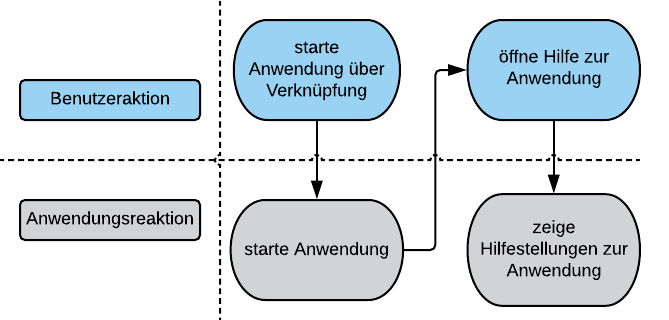
\includegraphics[width = 10cm]{Grafik/T010-Ablauf.png}
		\caption{Kurze Darstellung des Ablaufs von Testfall \textbf{T010}.}
		\label{T010-Ablauf}
	\end{center}
\end{figure}
\begin{itemize}

\item []\textbf{Testziel:} Teste das Verhalten der Anwendung aus der Sicht eines Benutzers, der diese zum ersten Mal verwendet. Der Ablauf ist in Abbildung \ref{T010-Ablauf} zu sehen.

\item []\textbf{Vorbedingung:} Die Anwendung ist installiert. Zu Sehen ist der Desktop des Benutzers mit einer Verknüpfung zur Anwendung.
\item []\textbf{Aktion:} Der Benutzer öffnet die Anwendung über die Verknüpfung. Danach informiert er sich über die Anwendung über die Hilfe in der Systemleiste.
\item []\textbf{Reaktion:} Die Anwendung öffnet sich. Zu Sehen ist das Hauptfenster mit leerem Konfigurationsfeld und leeren Darstellungen. Nach dem Öffnen der Hilfe, sieht der Benutzer die nötigen Informationen zur Bedienung der Anwendung. 
\item []\textbf{Nachbedingung:} Nach dem öffnen der Anwendung, überprüft diese, ob ein \gls{RasPi} angeschlossen ist. Jeder dargestellte Text ist auf Deutsch.

\item []\textbf{Ergebnis:} Der Benutzer kann die Anwendung starten. Die Bedienung der Anwendung ist komplett auf Deutsch möglich.
\item []\textbf{Wichtige abgedeckte Funktionale Anforderungen} \hyperlink{link-f010}{\textbf{F010}} erreiche GUI nach Start, \hyperlink{link-f140}{\textbf{F140}} leere Darstellung nach Anwendungsstart, \hyperlink{link-f480}{\textbf{F480}} Hilfe zu Anwendung, \hyperlink{link-f490}{\textbf{F490}} Texte der Anwendung auf Deutsch

\end{itemize}


\hypertarget{link-t020}{\item[\textbf{T020}]} Starten der Demo 

\begin{figure}[htbp]
	\begin{center}
		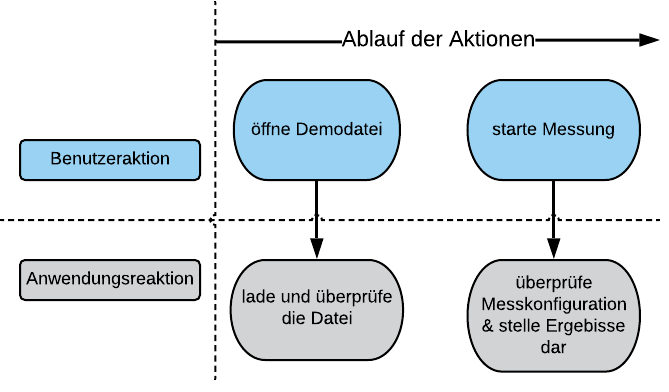
\includegraphics[width = 10cm]{Grafik/T020-Ablauf.png}
		\caption{Kurze Darstellung des Ablaufs von Testfall \textbf{T020}.}
		\label{T020-Ablauf}
	\end{center}
\end{figure}
\begin{itemize}

\item []\textbf{Testziel:} Teste das Verhalten der Anwendung beim Ausführen der Demo. Die Demo nutzt Daten aus einer Datei und benötigt keinen angeschlossenen \gls{RasPi}. Der Ablauf ist in Abbildung \ref{T020-Ablauf} zu sehen.

\item []\textbf{Vorbedingung:} Die Anwendung ist gestartet worden. Zu Sehen ist das offene Hauptfenster mit leerem Konfigurationsfeld.
\item []\textbf{Aktionen:} Der Benutzer öffnet die Messkonfigurationsdatei der Demo mit Hilfe der Ladefunktion der Systemleiste. Sobald die Messkonfiguration geladen ist, startet der Benutzer die Messung.
\item []\textbf{Reaktionen:} Nach dem Laden ist die Messkonfiguration in dem Konfigurationsfeld sichtbar. Nach dem Starten der Messung sieht der Benutzer wie die Daten im Graph dargestellt werden.
\item []\textbf{Nachbedingung:} Die Anwendung ist offen. Eine gültige Messkonfiguration ist in der Konfigurationsfeld geladen. Die Messung läuft ohne Fehler und die Ergebnisse werden richtig dargestellt.

\item []\textbf{Ergebnis:} Die Anwendung kann eine Messkonfiguration, die nur Daten aus einer Datei benötigt, problemlos ohne angeschlossenem \gls{RasPi} durchführen. 
\item []\textbf{Wichtige abgedeckte Funktionale Anforderungen, die in den vorangegangenen Testfällen noch nicht abgedeckt wurden:} \hyperlink{link-f130}{\textbf{F130}} Starten einer Messung, \hyperlink{link-f160}{\textbf{F160}} Laden einer Messkonfiguration

\end{itemize}



\hypertarget{link-t030}{\item[\textbf{T030}]} Lehrer erstellt und speichert eine Messkonfiguration

\begin{figure}[htbp]
	\begin{center}
		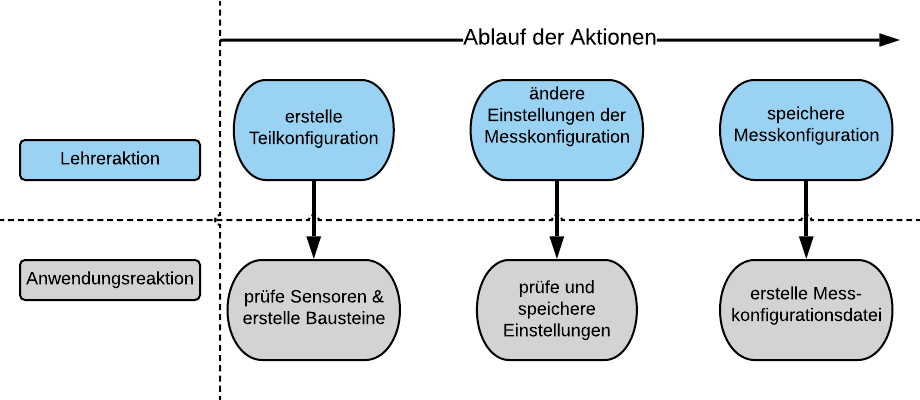
\includegraphics[width = 13cm]{Grafik/T030-Ablauf.png}
		\caption{Kurze Darstellung des Ablaufs von Testfall \textbf{T030}.}
		\label{T030-Ablauf}
	\end{center}
\end{figure}




\begin{itemize}

\item []\textbf{Testziel:} Teste eine typische Verwendung der Software anhand des gegebenen Szenarios. Dabei wird das Erstellen, Verändern und Speichern einer Messkonfiguration getestet. Der Ablauf ist in Abbildung \ref{T030-Ablauf} zu sehen.

\item []\textbf{Vorbedingung:} Die Anwendung ist gestartet und es liegt keine Messkonfiguration vor. Die Anwendung hat Zugriff auf einen laufenden \gls{RasPi} mit \gls{PhyPiDAQ}. Die Sensoren die verwendet werden sollen sind ordnungsgemäß angeschlossen.
\item []\textbf{Aktionen:} Der Lehrer zieht zwei angeschlossene Sensoren und eine Transformation in das Konfigurationsfeld. Danach ändert er einige Einstellungen an der Messkonfiguration. Das Ergebnis speichert er über die Systemleiste als Messkonfigurationsdatei.
\item []\textbf{Reaktion:} Nach jedem Hinzufügen eines Sensors oder einer Transformation, wird an der entsprechenden Stelle der jeweilige Konfigurationsbaustein sichtbar. Nach dem Speichern der Messkonfiguration sieht der Lehrer die erstellte Datei.
\item []\textbf{Nachbedingung:} Die Anwendung prüft beim Hinzufügen eines Sensorbausteins, ob der Sensor angeschlossen ist. Die Anwendung speichert die angepassten Einstellungen, sofern sie gültig sind. Die Messkonfigurationsdatei wird erstellt, unabhängig ob die Messkonfiguration vollständig oder gültig ist.

\item []\textbf{Ergebnis:} Die Anwendung kann eine Messkonfiguration als Datei speichern und prüfen, ob ein Sensor angeschlossen ist.
\item []\textbf{Wichtige abgedeckte funktionale Anforderungen, die in den vorangegangenen Testfällen noch nicht abgedeckt wurden:} \hyperlink{link-f180}{\textbf{F180}} füge Sensor hinzu, \hyperlink{link-f190}{\textbf{F190}} prüfe ob Sensor angeschlossen, \hyperlink{link-f210}{\textbf{F210}} füge Transformation hinzu, \hyperlink{link-f250}{\textbf{F250}} speichere Messkonfiguration, \hyperlink{link-f290}{\textbf{F290}} Einstellungen Messkonfiguration 

\end{itemize}

\hypertarget{link-t040}{\item[\textbf{T040}]} Schüler bearbeitet Aufgabe

\begin{figure}[htbp]
	\begin{center}
		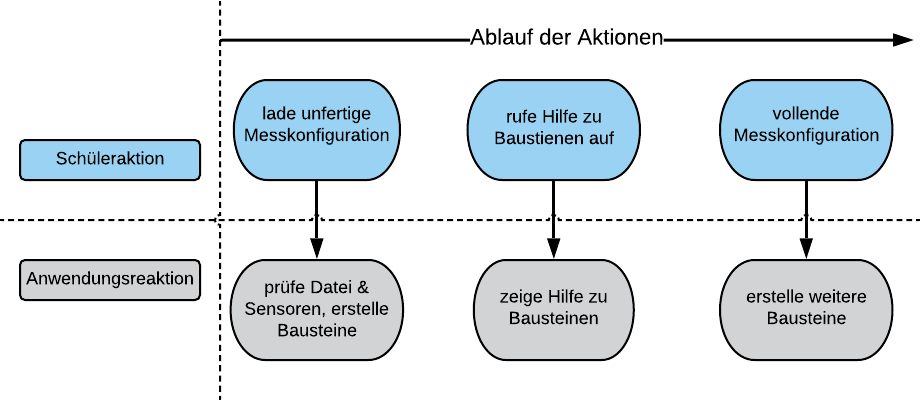
\includegraphics[width = 13cm]{Grafik/T040-Ablauf.png}
		\caption{Kurze Darstellung des Ablaufs von Testfall \textbf{T040}.}
		\label{T040-Ablauf}
	\end{center}
\end{figure}
\begin{itemize}

\item []\textbf{Testziel:} Teste die Anwendung aus Sicht eines Schülers, der eine Aufgabe bearbeiten soll.

\item []\textbf{Vorbedingung:} Die Anwendung ist gestartet und es liegt keine Messkonfiguration vor. Die Anwendung hat Zugriff auf einen laufenden \gls{RasPi} mit \gls{PhyPiDAQ}. Die Sensoren die verwendet werden sollen sind ordnungsgemäß angeschlossen. Der Ablauf ist in Abbildung \ref{T040-Ablauf} zu sehen.

\item []\textbf{Aktionen:} Der Schüler lädt über die Systemleiste die Messkonfiguration der Aufgabe. Danach informiert er sich über die Sensoren, Transformationen und Darstellungen über die angebotene Hilfestellungen. Als Nächstens vollendet er die Messkonfiguration.
 
\item []\textbf{Reaktionen:} Nach dem Laden sieht der Schüler die Messkonfiguration in dem Konfigurationsfeld. Wenn der Schüler die Hilfe aufruft, bekommt er die wesentlichen Informationen die er zur Verwendung der Anwendung braucht. Weiter sieht er, wie sich die graphische Darstellung der Messkonfiguration durch seine Aktionen verändert. 
\item []\textbf{Nachbedingung:} Die Anwendung prüft beim Laden der Messkonfiguration, ob die Sensoren angeschlossen sind. 


\item []\textbf{Ergebnis:} Der Benutzer kann Messkonfigurationen laden, diese verändern und durch das Erstellen auf Gültigkeit prüfen. 
\item []\textbf{Wichtige abgedeckte funktionale Anforderungen, die in den vorangegangenen Testfällen noch nicht abgedeckt wurden:} \hyperlink{link-f230}{\textbf{F230}} füge Darstellung hinzu, \hyperlink{link-f470}{\textbf{F470}} Hilfe Bausteine

\end{itemize}

\hypertarget{link-t050}{\item[\textbf{T050}]} Schüler startet Messung und speichert Ergebnisse

\begin{figure}[htbp]
	\begin{center}
		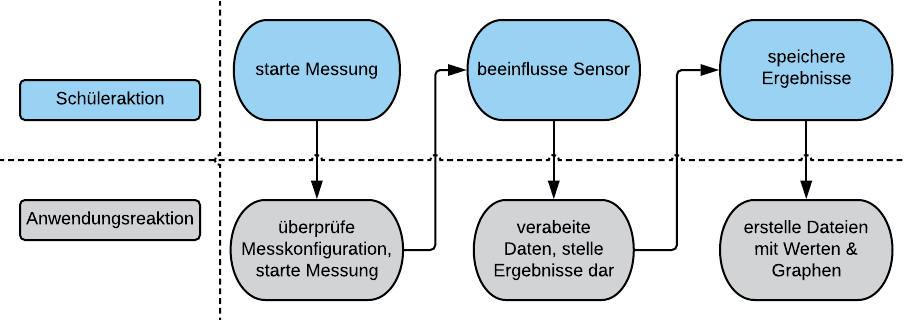
\includegraphics[width = 13cm]{Grafik/T050-Ablauf.png}
		\caption{Kurze Darstellung des Ablaufs von Testfall \textbf{T050}.}
		\label{T050-Ablauf}
	\end{center}
\end{figure}
\begin{itemize}

\item []\textbf{Testziel:} Teste die Anwendung aus Sicht eines Schülers, der Messung starten und deren Ergebnisse speichern soll. Der Ablauf ist in Abbildung \ref{T050-Ablauf} zu sehen.

\item []\textbf{Vorbedingung:} Die Anwendung ist gestartet und es ist die in \hyperlink{link-t040}{\textbf{T040}} erstelle Messkonfiguration geladen worden.

\item []\textbf{Aktionen:} Der Schüler startet die Messung. Während der Messung beeinflusst er die Daten durch einen Sensor. Am Ende der Messung speichert der Schüler den resultierenden Graphen und die Werte als Dateien ab.
\item []\textbf{Reaktionen:} Nach dem Starten, sieht er, wie die Daten als Graphen dargestellt werden. Außerdem sieht er, wie diese durch seine Aktionen verändert werden. Die Ergebnisse der Messung sieht er nach dem Speichern als erstellte Dateien.
\item []\textbf{Nachbedingung:} Die Anwendung prüft vor dem Starten der Messung, ob die Messkonfiguration gültig ist. Während die Messung läuft, werden die Daten verarbeitet und dargestellt unabhängig davon, ob der Schüler sie durch den Sensor beeinflusst. Die Ergebnisse sind zum Speichern verfügbar, sobald die Messung angehalten wurde.


\item []\textbf{Ergebnis:} Der Benutzer die Messung einer gültigen Messkonfiguration starten. Die Ergebnisse kann er als Graphen oder als Werte speichern. 
\item []\textbf{Wichtige abgedeckte funktionale Anforderungen, die in den vorangegangenen Testfällen noch nicht abgedeckt wurden:} \hyperlink{link-f300}{\textbf{F300}} Starte Messung, \hyperlink{link-f320}{\textbf{F320}} stelle Ergebnisse dar, \hyperlink{link-f400}{\textbf{F400}} speichere Messdaten, \hyperlink{link-f410}{\textbf{F410}} speichere Messgraph


\end{itemize}
\end{description}

\subsection{Testfälle zur Handhabung von Fehlern}

\begin{description} 

\hypertarget{link-t200}{\item[\textbf{T200}]} Laden einer ungültigen Datei als Messkonfiguration

\begin{figure}[htbp]
	\begin{center}
		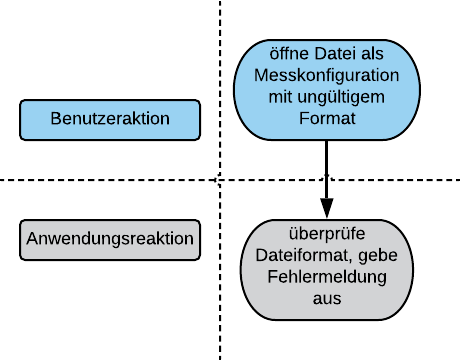
\includegraphics[width = 7cm]{Grafik/T200-Ablauf.png}
		\caption{Kurze Darstellung des Ablaufs von Testfall \textbf{T200}.}
		\label{T200-Ablauf}
	\end{center}
\end{figure}
\begin{itemize}

\item []\textbf{Testziel:} Teste das Verhalten der Anwendung beim Laden von ungültigen Messkonfigurationsdateien. Der Ablauf ist in Abbildung \ref{T200-Ablauf} zu sehen.

\item []\textbf{Vorbedingung:} Geöffnete Anwendung.
\item []\textbf{Aktionen:} Der Benutzer öffnet den Dialog zum Laden einer Datei über die Systemleiste und wählt eine Datei mit ungültigem Format zum Laden aus.
\item []\textbf{Reaktionen:} Eine aussagekräftige Fehlermeldung wird ausgegeben.
\item []\textbf{Nachbedingung:} Die Anwendung überprüft, ob die Datei ein gültiges Format hat und verhindert das Laden von ungültigen Formaten. 


\item []\textbf{Ergebnis:} Die Anwendung kann beim Laden von Messkonfigurationen zwischen gültigen und ungültigen Dateiformaten unterscheiden und entsprechend reagieren.
\item []\textbf{Wichtige abgedeckte funktionale Anforderungen, die in den vorangegangenen Testfällen noch nicht abgedeckt wurden:} \hyperlink{link-f430}{\textbf{F430}} überprüfe Format bei Laden

\end{itemize}

\hypertarget{link-t210}{\item[\textbf{T210}]} Erstellen einer ungültigen Messkonfiguration

\begin{figure}[htbp]
	\begin{center}
		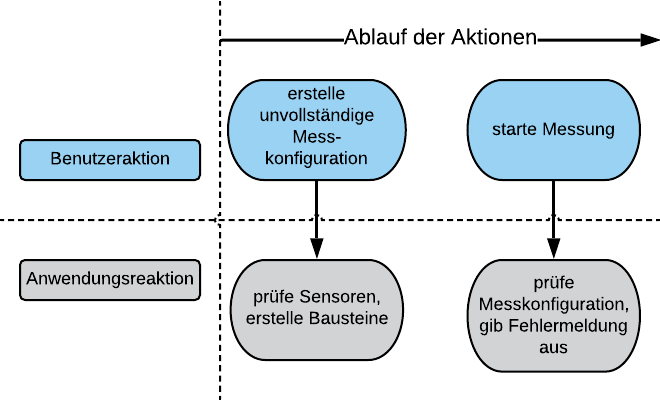
\includegraphics[width = 10cm]{Grafik/T210-Ablauf.png}
		\caption{Kurze Darstellung des Ablaufs von Testfall \textbf{T210}.}
		\label{T210-Ablauf}
	\end{center}
\end{figure}
\begin{itemize}

\item []\textbf{Testziel:} 

\item []\textbf{Vorbedingung:} Das Hauptfenster der Anwendung ist geöffnet. Die verwendeten Sensoren sind angeschlossen. Der Ablauf ist in Abbildung \ref{T210-Ablauf} zu sehen.

\item []\textbf{Aktionen:} Der Benutzer konstruiert eine Messkonfiguration aus zwei Sensoren, einer Transformation und einer Darstellung. Allerdings verbindet er die Darstellung nicht mit dem Rest der Konstruktion und startet die Messkonfiguration.
\item []\textbf{Reaktionen:} Die Messung wird nicht gestartet, sondern eine aussagekräftige Fehlermeldung wird ausgegeben.
\item []\textbf{Nachbedingung:} Die Anwendung überprüft vor dem Starten der Messkonfiguration, ob diese gültig ist.

\item []\textbf{Ergebnis:} Die Anwendung kann beim Starten zwischen gültigen und ungültigen Messkonfigurationen unterscheiden und entsprechend reagieren.
\item []\textbf{Wichtige abgedeckte funktionale Anforderungen, die in den vorangegangenen Testfällen noch nicht abgedeckt wurden:} \hyperlink{link-f310}{\textbf{F310}} überprüfe Messkonfiguration beim Start

\end{itemize}

\hypertarget{link-t220}{\item[\textbf{T220}]} Entfernen eines Sensors bei laufender Messung

\begin{figure}[htbp]
	\begin{center}
		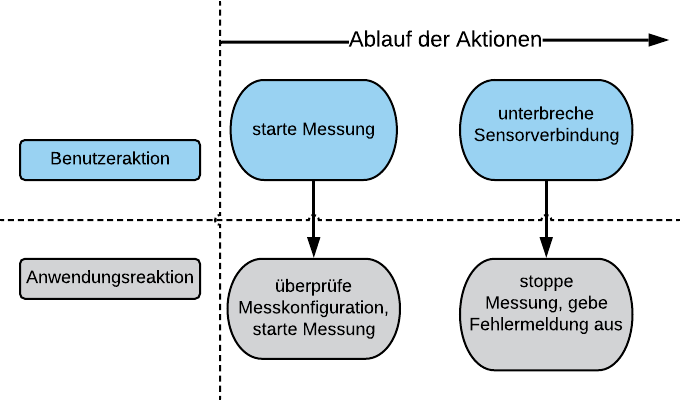
\includegraphics[width = 10cm]{Grafik/T220-Ablauf.png}
		\caption{Kurze Darstellung des Ablaufs von Testfall \textbf{T220}.}
		\label{T220-Ablauf}
	\end{center}
\end{figure}
\begin{itemize}

\item []\textbf{Testziel:} Teste das Verhalten der Anwendung, wenn ein Sensor ausfällt und dessen Datenstrom abbricht. Der Ablauf ist in Abbildung \ref{T220-Ablauf} zu sehen.

\item []\textbf{Vorbedingung:} Die Anwendung ist geöffnet. Alle verwendeten Sensoren sind angeschlossen und betriebsbereit. Eine gültige Messkonfiguration aus zwei Sensoren, einer Transformation und einer Darstellung wurde geladen.
\item []\textbf{Aktionen:} Der Benutzer startet die Messung. Aus einem unbekannten Grund wird die Verbindung zu einem Sensor getrennt.
\item []\textbf{Reaktionen:} Die Messung stoppt. Eine aussagekräftige Fehlermeldung wird ausgegeben.
\item []\textbf{Nachbedingung:} \gls{PhyPiDAQ} verliert die Verbindung zu einem Sensor und sendet keine Daten mehr an die Anwendung. Die Anwendung stürzt nicht ab, sondern gibt eine Fehlermeldung aus.

\item []\textbf{Ergebnis:} Die Anwendung kann mit dem ungewollten Verlust eines Datenstroms umgehen ohne abzustürzen.
\item []\textbf{Wichtige abgedeckte funktionale Anforderungen, die in den vorangegangenen Testfällen noch nicht abgedeckt wurden:} \hyperlink{link-f450}{\textbf{F450}} Melde Abbruch des Datenstrom

\end{itemize}


\end{description}


\section{Szenario mit Use-case-Diagramm}\label{scenario}

Abbildung \ref{UseCaseDiagramm} zeigt die Use-Cases und deren Ablauf für das nun im Folgenden beschriebene Szenario. Akteure in diesem Szenario sind ein Lehrer, ein Schüler sowie ein weiterer Lehrer. Das Szenario verwendet weitestgehend Testfälle aus Kapitel \ref{testfall}. (Bausteinprototypen sind lediglich in Sollkriterien spezifiziert und werden von den Testfällen in Kapitel \ref{testfall} nicht abgedeckt.)

\begin{enumerate}
	\item Lehrer A kennt das Messkonfigurationswerkzeug noch nicht so gut und erstellt zunächst eine ungültige \gls{Benutzerkonfiguration}. 
	
	\item Der zweite Versuch gelingt und Lehrer A erstellt erfolgreiche eine Messkonfiguration, die sich gut als Basis für seinen Unterricht eignet. Diese Messkonfiguration speichert er sogleich auf seinem Speicherstick.
	
	\item Am nächsten Tag gibt Lehrer A den Speicherstick einem seiner Schüler. 
	
	\item Dieser soll die vorbereitete Aufgabe bearbeiten. Also öffnet er die Messkonfiguration und bearbeitet diese.
	
	\item Da Lehrer A zunächst Zweifel hat, dass sein Schüler die Aufgabe ordnungsgemäß gelöst hat, lässt er ihn einen Messlauf durchführen. Der Messlauf verläuft wie erwartet, und weil der Schüler sehr ordentlich ist, speichert er die Messergebnisse.
	
	\item Es hat sich herumgesprochen, dass die Schüler von Lehrer A ganz begeistert von seinem Physik-Unterricht sind, und deshalb möchte Lehrer B einen ähnlichen Unterricht machen. Da er nicht so wie Lehrer A bei Null anfangen möchte, lässt er sich die eingangs von Lehrer A erstellte Messkonfiguration auf einem Speicherstick geben. 
	
	\item Lehrer B öffnet die Messkonfiguration und schaut sie sich genau an.
	
	\item Die Messkonfiguration enthält zwar einen brauchbaren Darstellungsbaustein. Da Lehrer B aber ein paar sehr schwache Schüler in seiner Klasse hat, möchte ein paar Aspekte auf den Darstellungen, die er erhält, besser hervorheben. Und er sieht schon kommen, dass er (und evtl. auch seine Kollegen) in Zukunft noch öfter von der verbesserten Darstellungsart profitieren könnten. Also erstellt er einen neuen optimierten Bausteinprototyp für Darstellungen.
	
	\item Lehrer B ersetzt den alten Darstellungsbaustein durch einen mit der verbesserten Darstellungsart. 
	
	\item Da die neue Darstellungsart auch in Zukunft noch öfter zum Einsatz kommen soll, speichert Lehrer B sie persistent. 
	
	\item Im darauffolgenden Schuljahr bekommt Lehrer A wieder eine Klasse der gleichen Klassenstufe zugewiesen, und dieses Mal hat auch er das Pech, ein paar sehr schwache Schüler in seiner Klasse zu haben. Er erzählt Lehrer B davon, und dieser überlässt ihm per Speicherstick eine Kopie der Datei, welche den bereits vor einem Jahr erstellten Bausteinprototypen enthält. 	
	
	\item Lehrer A öffnet die Datei und erkennt, dass die neuen Darstellungsbausteine, die er seinen Messkonfigurationen nun hinzufügen kann, sehr viel anschaulicher sind.
\end{enumerate}


\begin{figure}[h]
	\begin{center}
		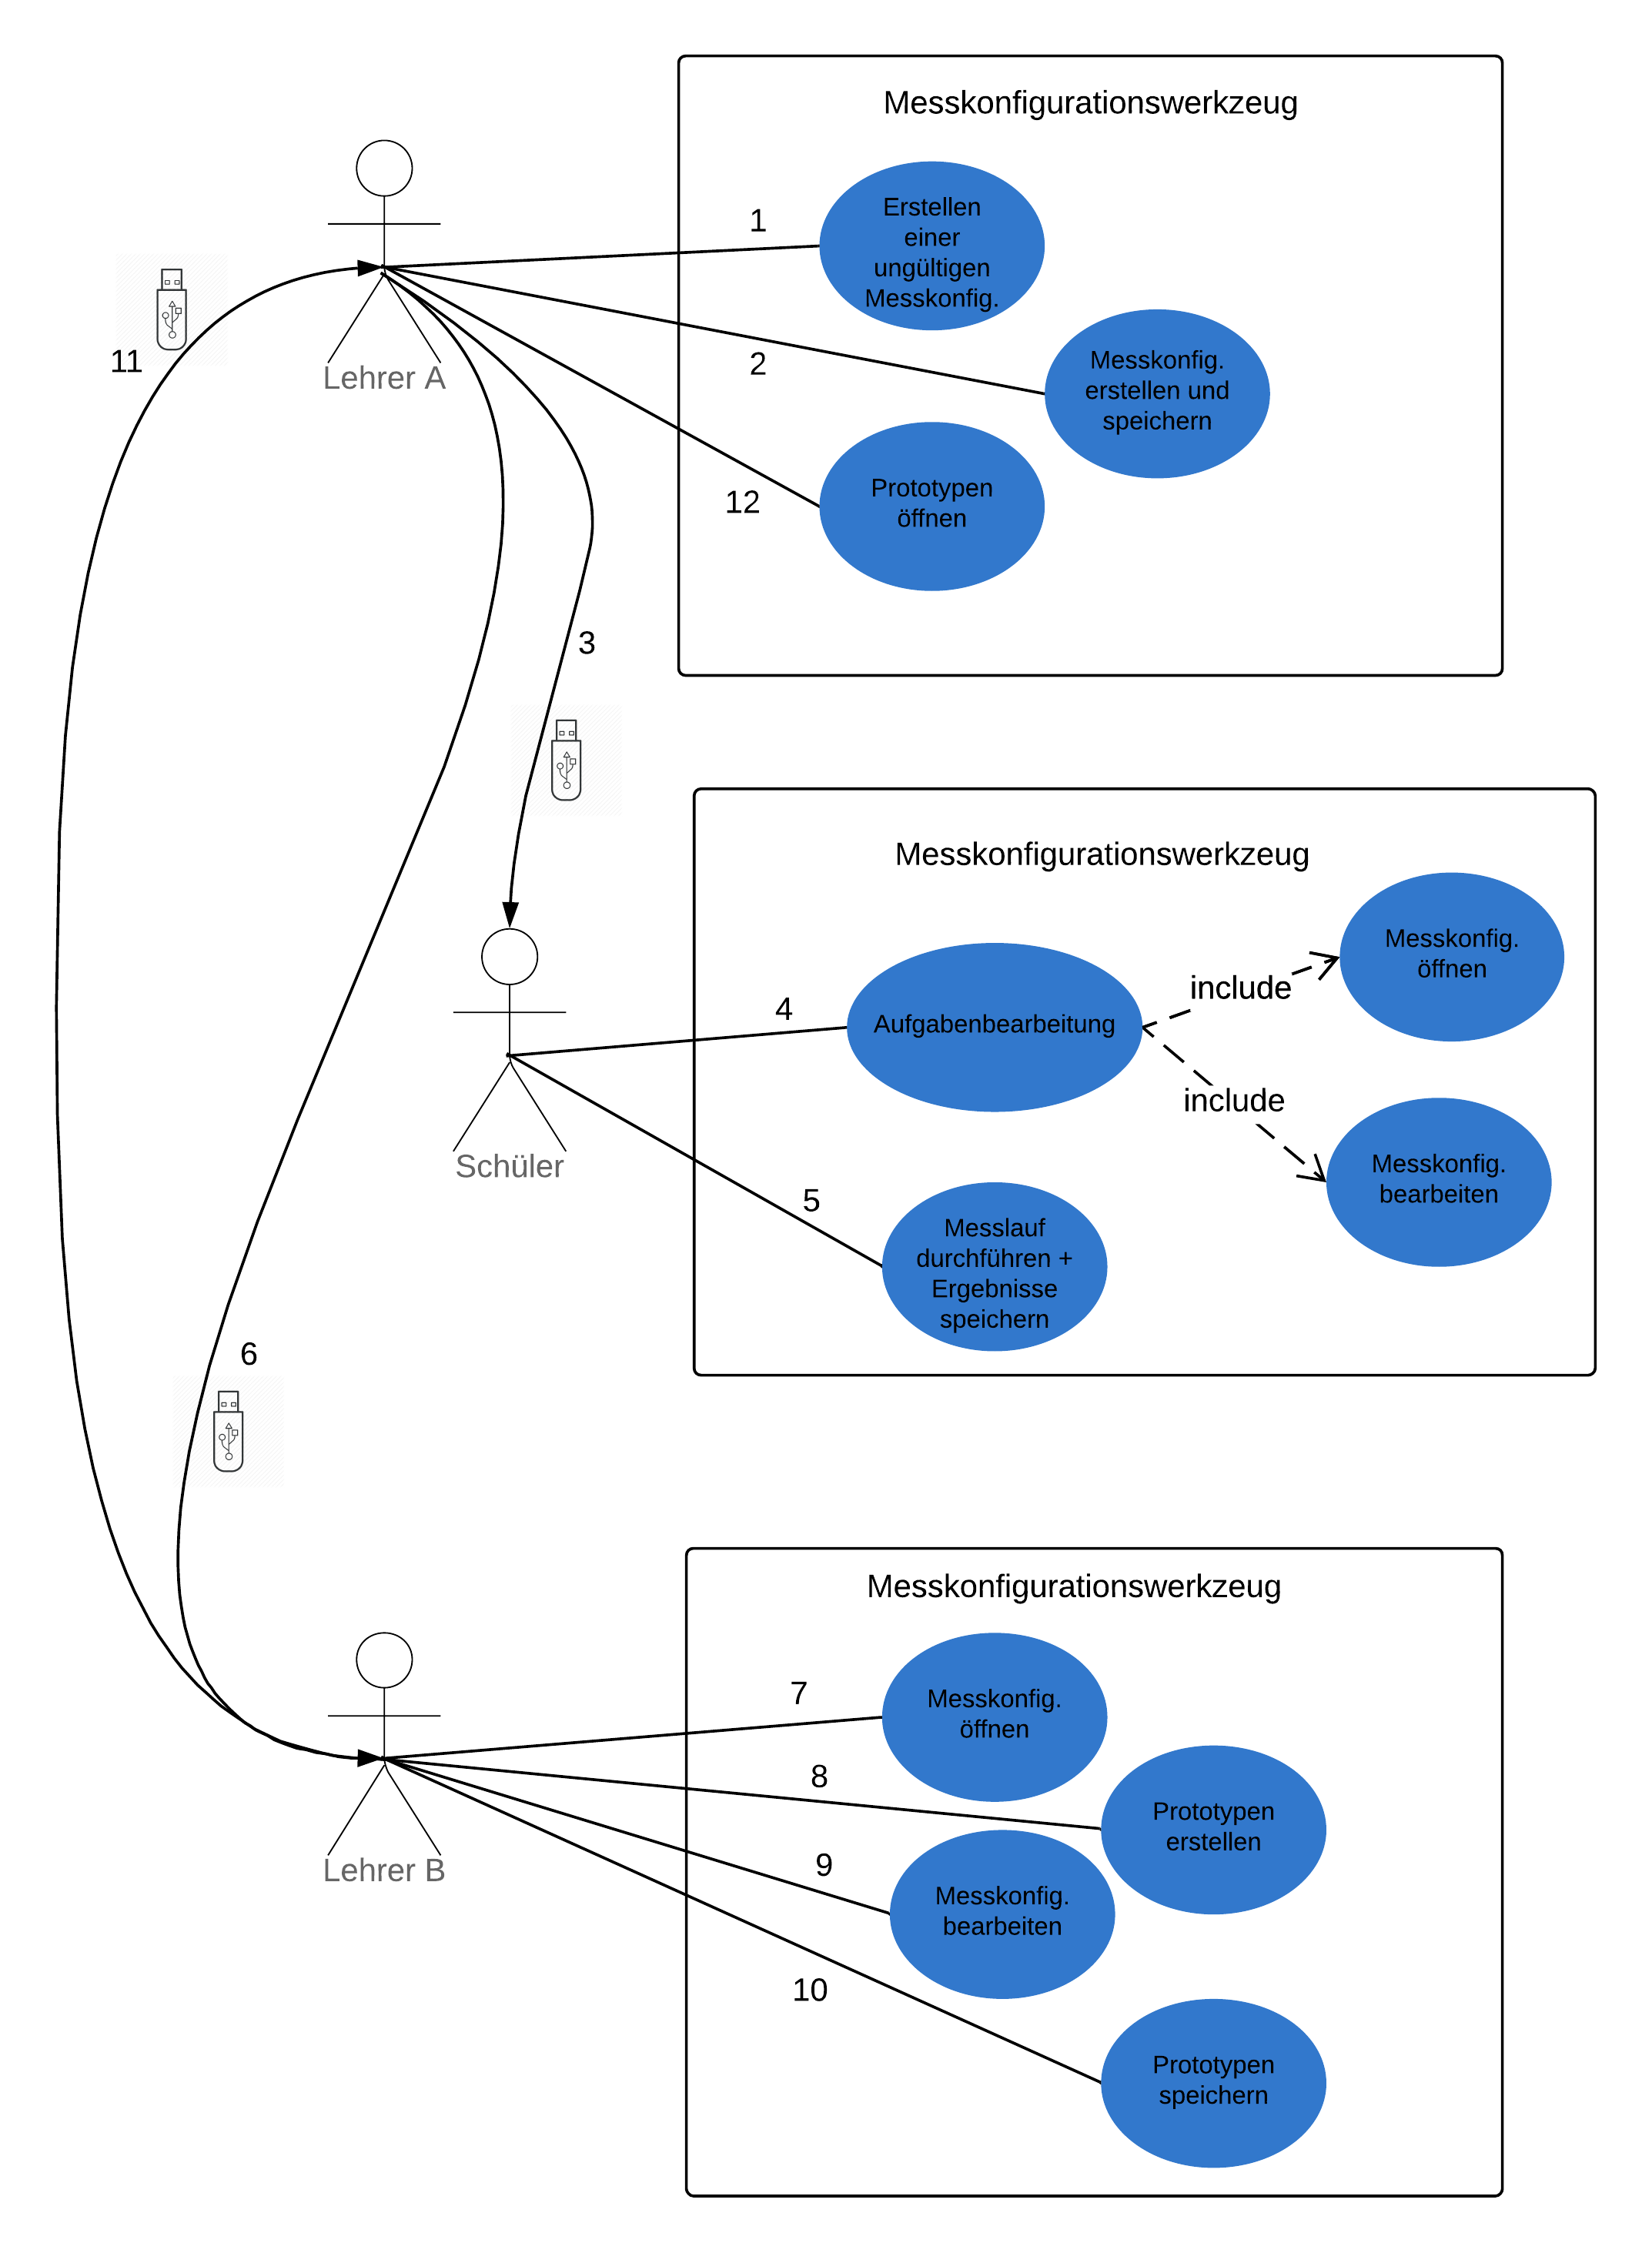
\includegraphics[width = 12cm]{Grafik/UseCaseDiagram.png}
		\caption{Use-Case-Diagramm}
		\label{UseCaseDiagramm}
	\end{center}
\end{figure}

\clearpage
\section{Systemmodelle}\label{systemmodell}

Das projektierte Gesamtsystem wird aller Voraussicht nach drei Systemprozesse benötigen, die wie in Abbildung \ref{DeploymentDiagram} dargestellt, miteinander Daten austauschen.

Einer dieser drei Systemprozesse hostet die \gls{JVM}, auf der die zu erstellende Hauptkomponente läuft. Diese enthält die grafische Benutzungsoberfläche, die im Wesentlichen die Erstellung der Werte verarbeitenden Messkonfiguration ermöglicht, und die auch deren Betrieb darstellen kann. 

Zum Ansteuern und Auslesen der Sensoren auf dem \gls{RasPi} wird das auf Python basierende Framework \gls{PhyPiDAQ} bereitgestellt. Dieses unterstützt bereits eine  ganze Reihe von Sensoren zur Messung diverser physikalischer Größen der Mechanik, Thermodynamik und Elektrodynamik. Da der Python-Interpreter im Allgemeinen nicht im selben Systemprozess wie die \gls{JVM} ausgeführt werden kann, wird für diesen ein zweiter Systemprozess benötigt.

Um Ressourcenknappheit auf dem \gls{RasPi} aus dem Weg zu gehen, aber auch zur Vereinfachung von Entwicklung und Demonstration, soll die Hauptkomponente nicht zwingend ebenso auf dem \gls{RasPi} ausgeführt werden müssen. 

Falls denn nun die Hauptkomponente tatsächlich auf einem anderen Rechner ausgeführt werden sollte, so muss sie mit dem Python-Interpreter hardware- bzw. plattformübergreifend Daten austauschen können. Bisher stellt PhyPiDAQ hierfür jedoch keine Funktionalität zur Verfügung.

Zur Realisierung der hardwareübergreifenden Kommunikation sind die folgenden zwei Lösungsvarianten denkbar: 

\begin{itemize}


	\item PhyPiDAQ wird um eine Kommunikationsschnittstelle erweitert, beispielsweise zur Kommunikation über eine Netzwerkschnittstelle wie z. B. WLAN oder zur Kommunikation über eine Peripherieschnittstelle wie z. b. USB.
	
%	\item In einem dritten Systemprozess, der auf dem selben Rechner wie PhyPiDAQ läuft, stellt eine Utility-Softwarekomponente einen entsprechenden Kommunikationsdienst bereit. In diesem Fall sollte keine Notwendigkeit bestehen, dass PhyPiDAQ wesentlich erweitert werden muss, und der Datenaustausch mit PhyPiDAQ sollte auf möglichst einfache Art und Weise, beispielsweise per Standardeingabe und Standardausösungsvariante erfolgen können.

\end{itemize}

Da bei letzterer Variante die Utility-Softwarekompomente zusätzlich auch noch eine Überwachungsfunktion bezüglich PhyPiDAQ übernehmen und dieses im Falle von Abstürzen und Nicht-Responsivität erneut ausführen kann, ist letztere Lösungsvariante die bevorzugte Lösungsvariante zur Realisierung der optionalen hardwareübergreifenden Kommunikation. 

Abbildung \ref{DeploymentDiagram} stellt die Verteilung der Systemkomponenten auf zwei Rechnern mittels der gewählten zweiten Lösungsvariante dar, und benennt die notwendige Utility-Komponente mit ,,Measurement-Server``. 
 

\begin{figure}[h]
	\begin{center}
		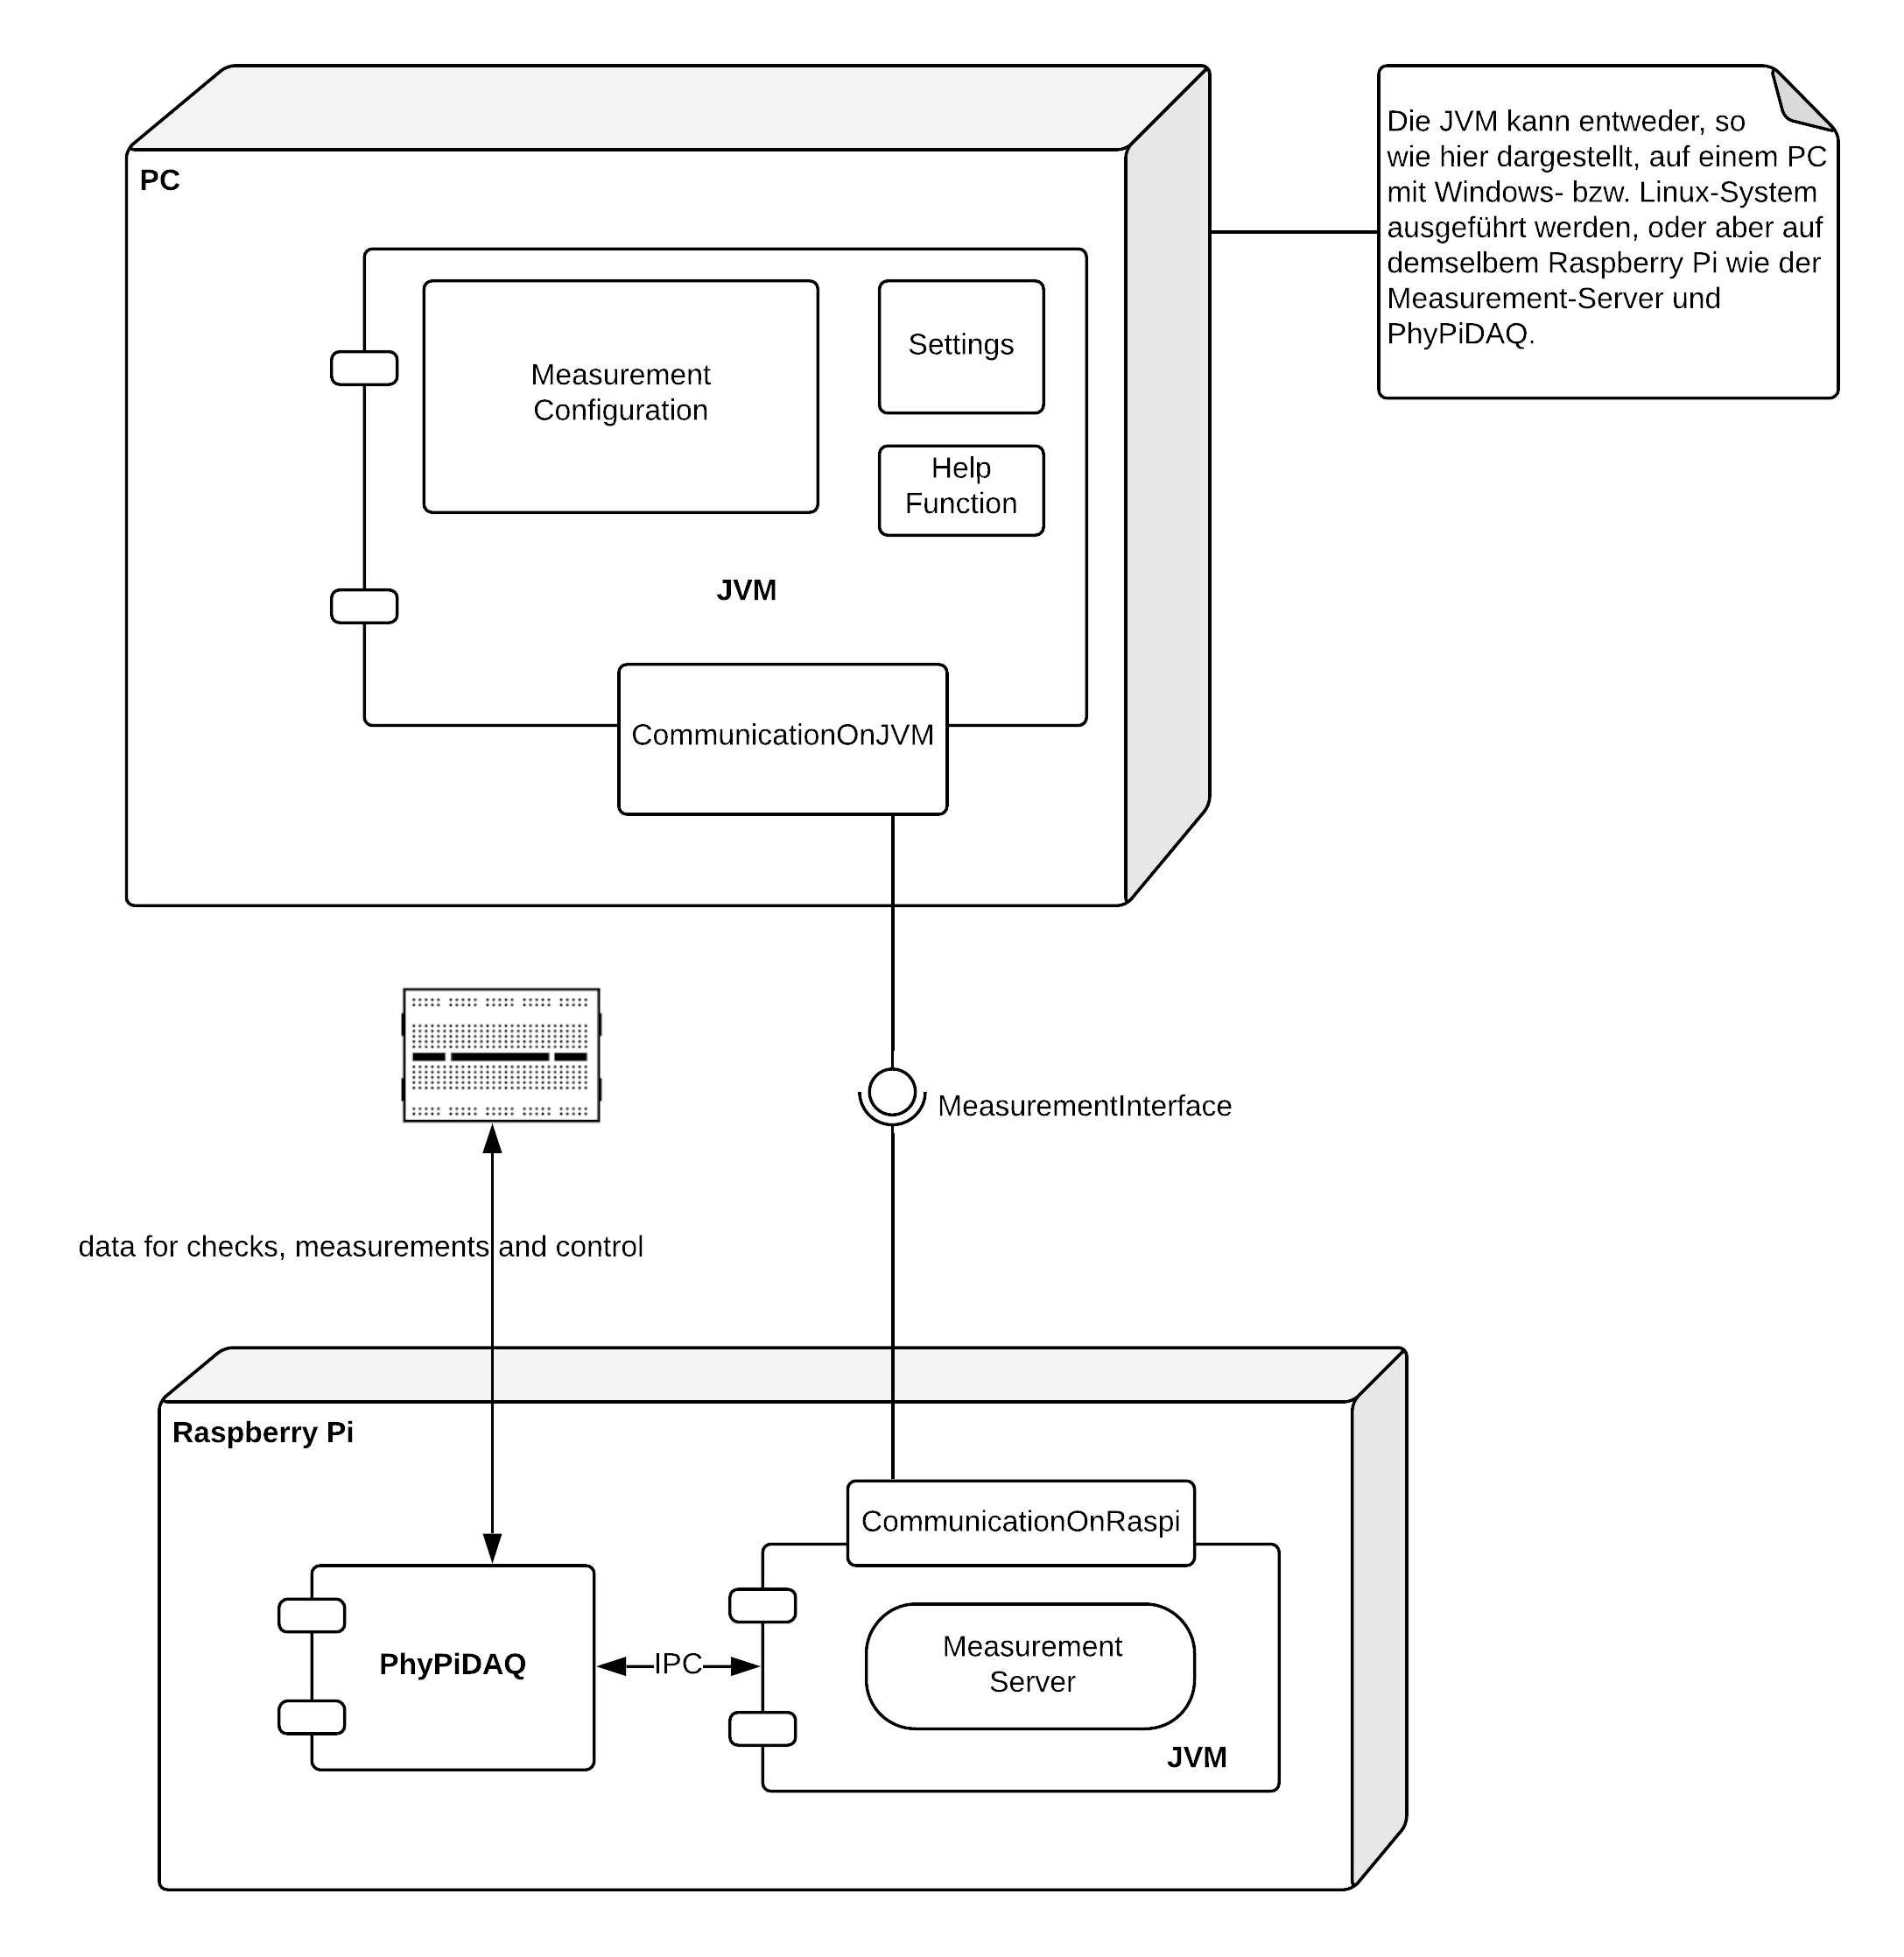
\includegraphics[width = 12cm]{Grafik/DeploymentDiagram.png}
		\caption{UML-Deployment-Diagramm}
		\label{DeploymentDiagram}
	\end{center}
\end{figure}

\clearpage
\section{Benutzungsoberfläche}\label{gui}

\subsection{Ziel der Benutzeroberfläche}

Das Ziel der Benutzeroberfläche ist es dem Anwender eine intuitive Benutzung des Programmes zu ermöglichen. Da das Programm im Schulbetrieb eingesetzt werden soll ist eine gute Verständlichkeit wichtig. So soll auch eine lange Einarbeitungszeit für den Anwender vermieden werden. Dabei soll keine Funktionalität verloren gehen.

\subsection{Generell}

Um die Ziele zu erfüllen wird das Programm über eine \gls{GrafBenOber}) (kurz ,,GUI``) bedient. Der Anwender soll in der Lage sein bereits vorhandene Computer und Mobilgerät Kenntnisse zu nutzen.

\subsection{Eingabegeäte}

Die \gls{GrafBenOber} soll Maus und Tastatureingaben unterstützen. Außerdem soll eine \gls{dragdrop} Eingabe möglich sein.
Die Verwendung anderer Eingabegeräte ist nicht vorgesehen.

\subsection{Überblick}

\begin{figure}[htbp]
	\begin{center}
		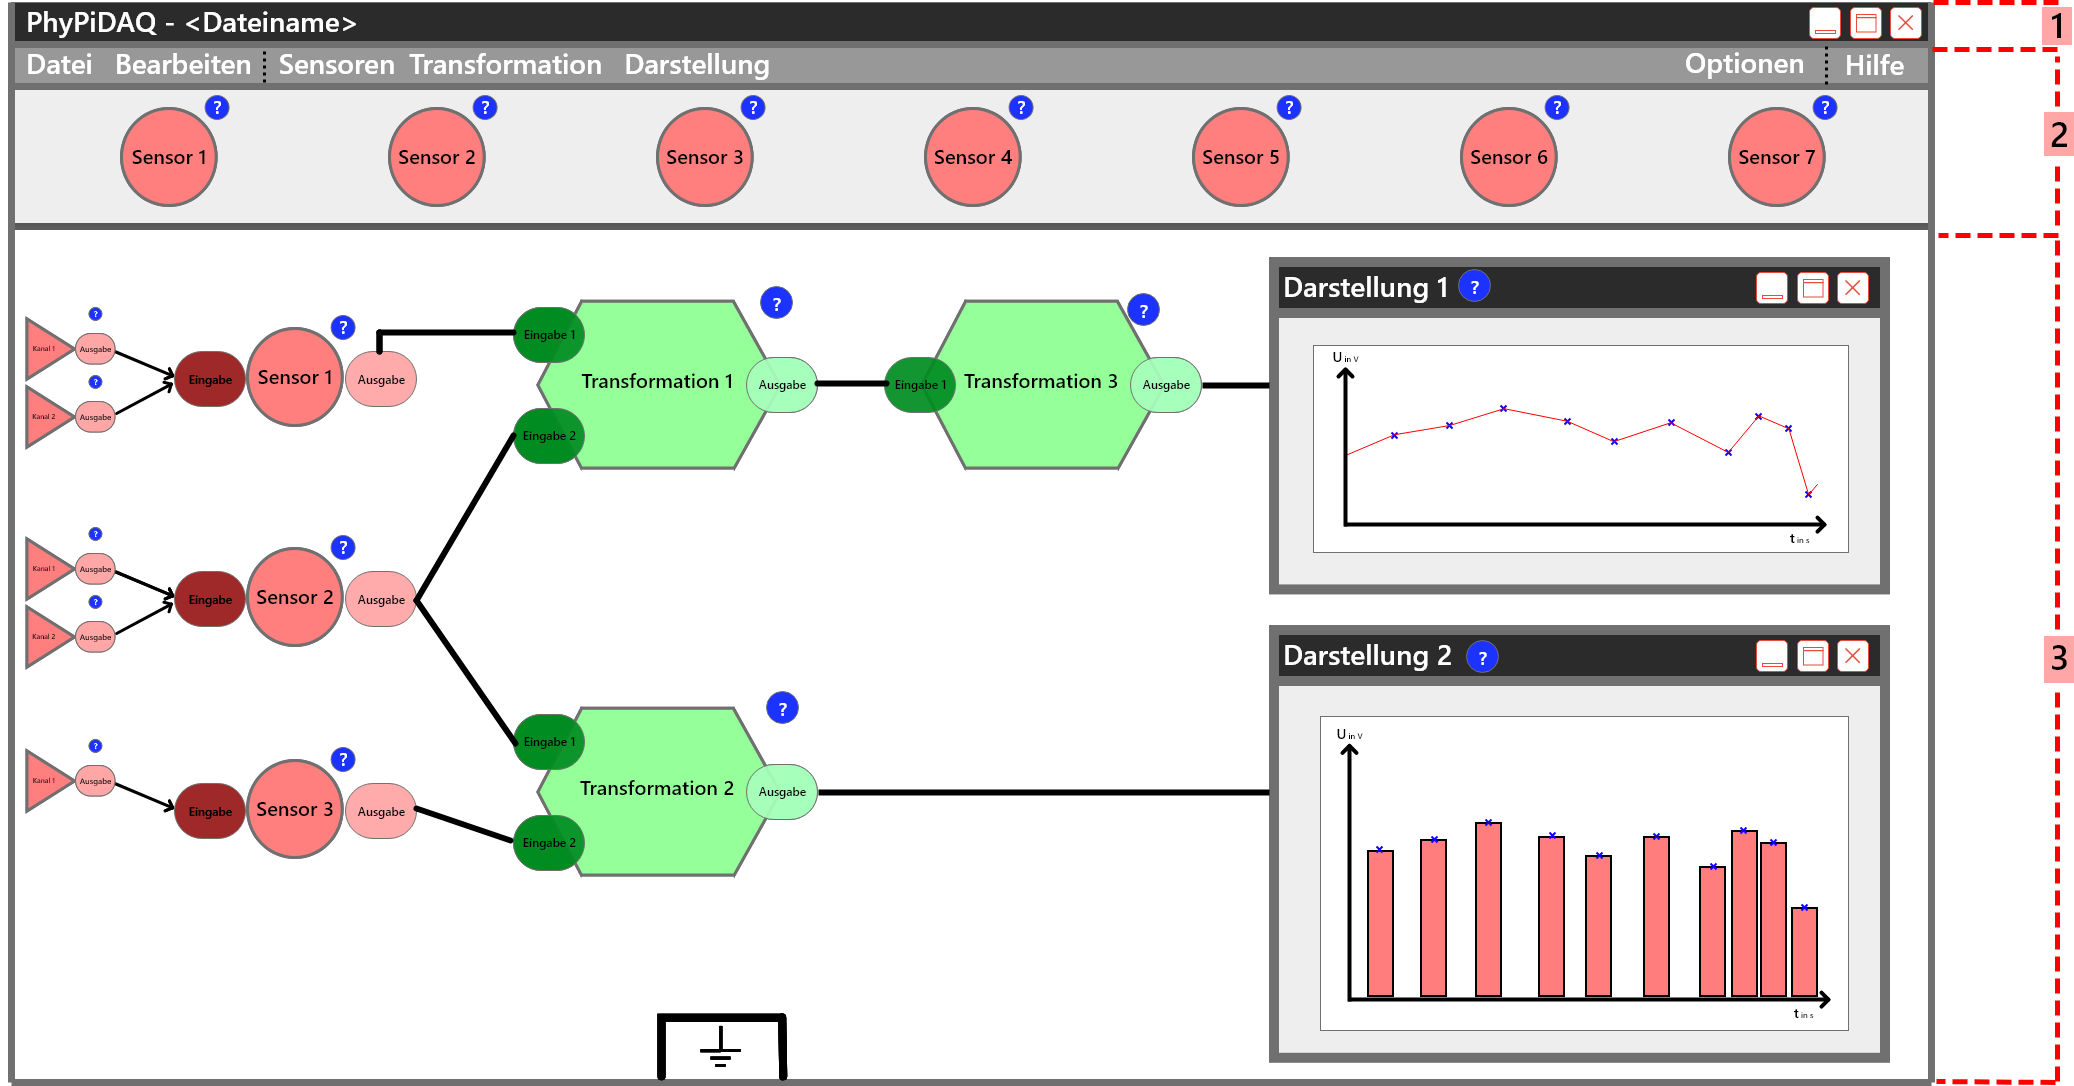
\includegraphics[width = 11cm]{Grafik/GUI-mit-Segmenten.png}
		\caption{Der Grundlegende Aufbau der Hauptbenutzeroberfläche}
		\label{GUI_Grundlage}
	\end{center}
\end{figure}

Abbildung \ref{GUI_Grundlage} zeigt den Aufbau einer möglichen \gls{GrafBenOber}. Dabei geben die Zahlen in den roten Kästchen, rechts von dem Programmfenster, die logische Unterteilung an.

Das Design der Einzelnen Elemente kann sich im Verlauf der Anwendungsentwicklung ändern. Die Grundlegenden Bausteine der \gls{GrafBenOber} werden sich in ihrer Aufgabe nicht ändern. Zu ihnen gehören:

\begin{itemize}
	\item \glspl{sensor}
	\item \glspl{transformation}
	\item \glspl{darstellung}
\end{itemize}

Die zu dem jeweiligen logischen Teil gehörenden Elemente sollen im folgenden erklärt werden.

\subsection{Element Beschreibungen}

\subsubsection{Systemmenüleiste}

In der Systemmenüleiste befinden sich Funktionen, die Einfluss auf die gesamte \gls{GrafBenOber} haben.

\begin{tabular}[t]{p{1cm} p{10cm}} %Alle Systemmenübausteine in einer Tabelle
	\vspace{0cm}
\includegraphics[width = 1 cm]{Grafik/PhyPiDAQ.png} & Der Name des Programmes wird hier angezeigt. Rechts daneben steht, sofern vorhanden, der Name der Datei, die gerade geöffnet ist.\newline\\
	\vspace{0cm}
\includegraphics[width = 1 cm]{Grafik/Maximieren.png} & Das ''Maximieren''-Symbol vergrößert das Programmfenster auf die maximale Größe. Die Größe ist von der Benutzungsumgebung abhängig.\newline\\
	\vspace{0cm}
\includegraphics[width = 1 cm]{Grafik/Minimieren.png} & Das ''Minimieren''-Symbol blendet das Programmfenster aus. Es ist weiterhin geöffnet und wieder aufrufbar. \\
	\vspace{0cm}
\includegraphics[width = 1 cm]{Grafik/Schliessen.png} & Das ''Schließen''-Symbol beendet die Anwendung. Vor dem Beenden findet eine Abfrage statt, ob der Anwender eventuell vorgenommene Änderungen speichern möchte.\\
\end{tabular}

\subsubsection{Auswahl}

In der Auswahl befinden sich Funktionen, die das Bearbeiten des Konfigurationsfeldes ermöglichen.

\begin{tabular}[t]{p{1cm} p{10cm}} %Auswahlelemente Teil 1
	\vspace{0cm}
\includegraphics[width = 1 cm]{Grafik/Datei.png} & Der Benutzer hat die Möglichkeit Dateien zu bearbeiten. Die wichtigsten Funktionen sind:
	\begin{itemize} 
		\item Das anlegen einer neuen Datei
		\item Das Speichern der aktuellen Datei
		\item Das Öffnen einer bereits erstellten Datei
	\end{itemize}\\
\end{tabular}

\begin{tabular}[t]{p{1cm} p{10cm}} %Auswahlelemente Teil 2
	\vspace{0cm}
\includegraphics[width = 1 cm]{Grafik/Bearbeiten.png} & Der Benutzer hat die Möglichkeit den Inhalt der aktuell geöffneten Datei zu bearbeiten. Die wichtigsten Funktionen sind:
	\begin{itemize} 
		\item Das Kopieren eines ausgewählten Objektes
		\item Das Einfügen eines gespeicherten Objektes
		\item Das Anpassen eines ausgewählten Elements. Diese Einstellungsmöglichkeiten sind von dem Objekt abhängig.
	\end{itemize}
\end{tabular}

\begin{tabular}[t]{p{1cm} p{10cm}} %Auswahlelemente Teil 3
	\vspace{0cm}
\includegraphics[width = 1 cm]{Grafik/Sensor.png} & Der Benutzer kann sich eine Auswahl von \glspl{sensor} anzeigen lassen. Die \glspl{sensor} können anschließend in das Konfigurationsfeld eingefügt werden. Die angezeigte Auswahl ist unabhängig von den angeschlossenen Sensoren\newline
\end{tabular}

\begin{tabular}[t]{p{1cm} p{10cm}} %Auswahlelemente Teil 4
	\vspace{0cm}
\includegraphics[width = 1 cm]{Grafik/Verbindung.png} & Der Benutzer kann sich eine Auswahl von \glspl{transformation} anzeigen lassen. Die \glspl{transformation} können anschließend per \gls{dragdrop} in das Konfigurationsfeld gezogen werden. Die Auswahl kann unter Optionen erweitert werden.\newline\\
	\vspace{0cm}
\includegraphics[width = 1 cm]{Grafik/Darstellung.png} & Der Benutzer kann sich eine Auswahl von \glspl{darstellung} anzeigen lassen. Die \glspl{darstellung} können anschließend in das Konfigurationsfeld eingefügt werden. Die Auswahl kann erweitert werden.\newline
\end{tabular}

\begin{tabular}[t]{p{1cm} p{10cm}} %Auswahlelemente Teil 5
	\vspace{0cm}
\includegraphics[width = 1 cm]{Grafik/Optionen.png} & Der Benutzer kann sich eine Auswahl an Optionen anzeigen lassen. Beispiele hierfür sind
	\begin{itemize} 
		\item Das Ändern von angezeigten Farben
		\item Das Erweitern der Transformations- und Darstellungsauswahl
	\end{itemize}\\
	\vspace{0cm}
\includegraphics[width = 1 cm]{Grafik/Hilfe.png} & Der Benutzer kann sich eine allgemeine Hilfe anzeigen lassen. In der Hilfe werden die Funktionen der Anwendung erklärt.\newline
\end{tabular}

Im Laufe der Entwicklung kann es sich als sinnvoll herausstellen weitere Optionen einzufügen bzw. bestehende Optionen zusammenzufügen.

\subsubsection{Konfigurationsfeld}

In dem Konfigurationsfeld wird die Messkonfiguration, des Anwenders, aufgebaut.

\begin{tabular}[t]{p{1cm} p{10cm}}
	\vspace{0cm}
\includegraphics[width = 1 cm]{Grafik/Information.png} & Das ''Informations''-Symbol zeigt nach einem Click weiterführende Informationen zu dem Element an, zu dem es gehört. So würde beispielsweise bei einer Transformation die Funktion angezeigt werde, die sie realisiert.\newline\\\cline{1-2}
	\vspace{0cm}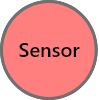
\includegraphics[width = 1 cm]{Grafik/Sensorelement.png} & Repräsentation eines Sensors, der in PhyPiDAQ erkannt werden kann. Voraussetzung hierfür ist die Existenz einer \gls{konfigdata}.\newline\\
	\vspace{0cm}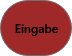
\includegraphics[width = 1 cm]{Grafik/Eingabe-Sensor.png} & Die zu einem Sensor gehörende Eingabe. Die Eingabe wird nur angezeigt, wenn auch die Kanäle angezeigt werden.\newline\\
	\vspace{0cm}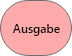
\includegraphics[width = 1 cm]{Grafik/Ausgabe-Sensor.png} & Die zu einem Sensor gehörende Ausgabe. Jeder Sensor hat genau eine Ausgabe.\newline\\
	\vspace{0cm}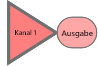
\includegraphics[width = 1 cm]{Grafik/Kanal.png} & Der zu einem Sensor gehörende Kanal. Die Anzahl an angezeigten Kanlälen hängt von dem Sensor ab. In den Optionen kann eingestellt werden, ob die Kanäle angezeigt werden.\newline\\\cline{1-2}
	\vspace{0cm}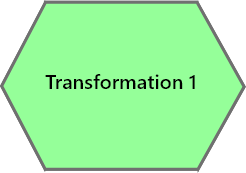
\includegraphics[width = 1 cm]{Grafik/Verbindungselement.png} & Repräsentation einer \gls{transformation}. Jedem Eingang können durch Einfügen von einer Verbindung Daten übergeben werden.\newline\\
	\vspace{0cm}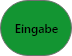
\includegraphics[width = 1 cm]{Grafik/Eingabe-Verbindung.png} & Die Eingabe einer Transformation. Die Anzahl der verfügbaren Eingaben hängt von der Transformation ab.\newline\\
	\vspace{0cm}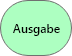
\includegraphics[width = 1 cm]{Grafik/Ausgabe-Transformation.png} & Die Ausgabe einer Transformation. Die Anzahl der verfügbaren Ausgaben hängt von der Transformation ab.\newline\\\cline{1-2}
	\vspace{0cm}
\includegraphics[width = 1 cm]{Grafik/Verbindungspfeil.png} & Eine Verbindung zwischen zwei Elementen. Sie besitz eine Richtung. Daten ''fließen'' also nicht in beide Richtungen.\newline\\
\end{tabular}

\clearpage

\subsection{Erweiterungsmöglichkeiten}

\subsubsection{Startbildschirm}

\begin{figure}[htbp]
	\begin{center}
		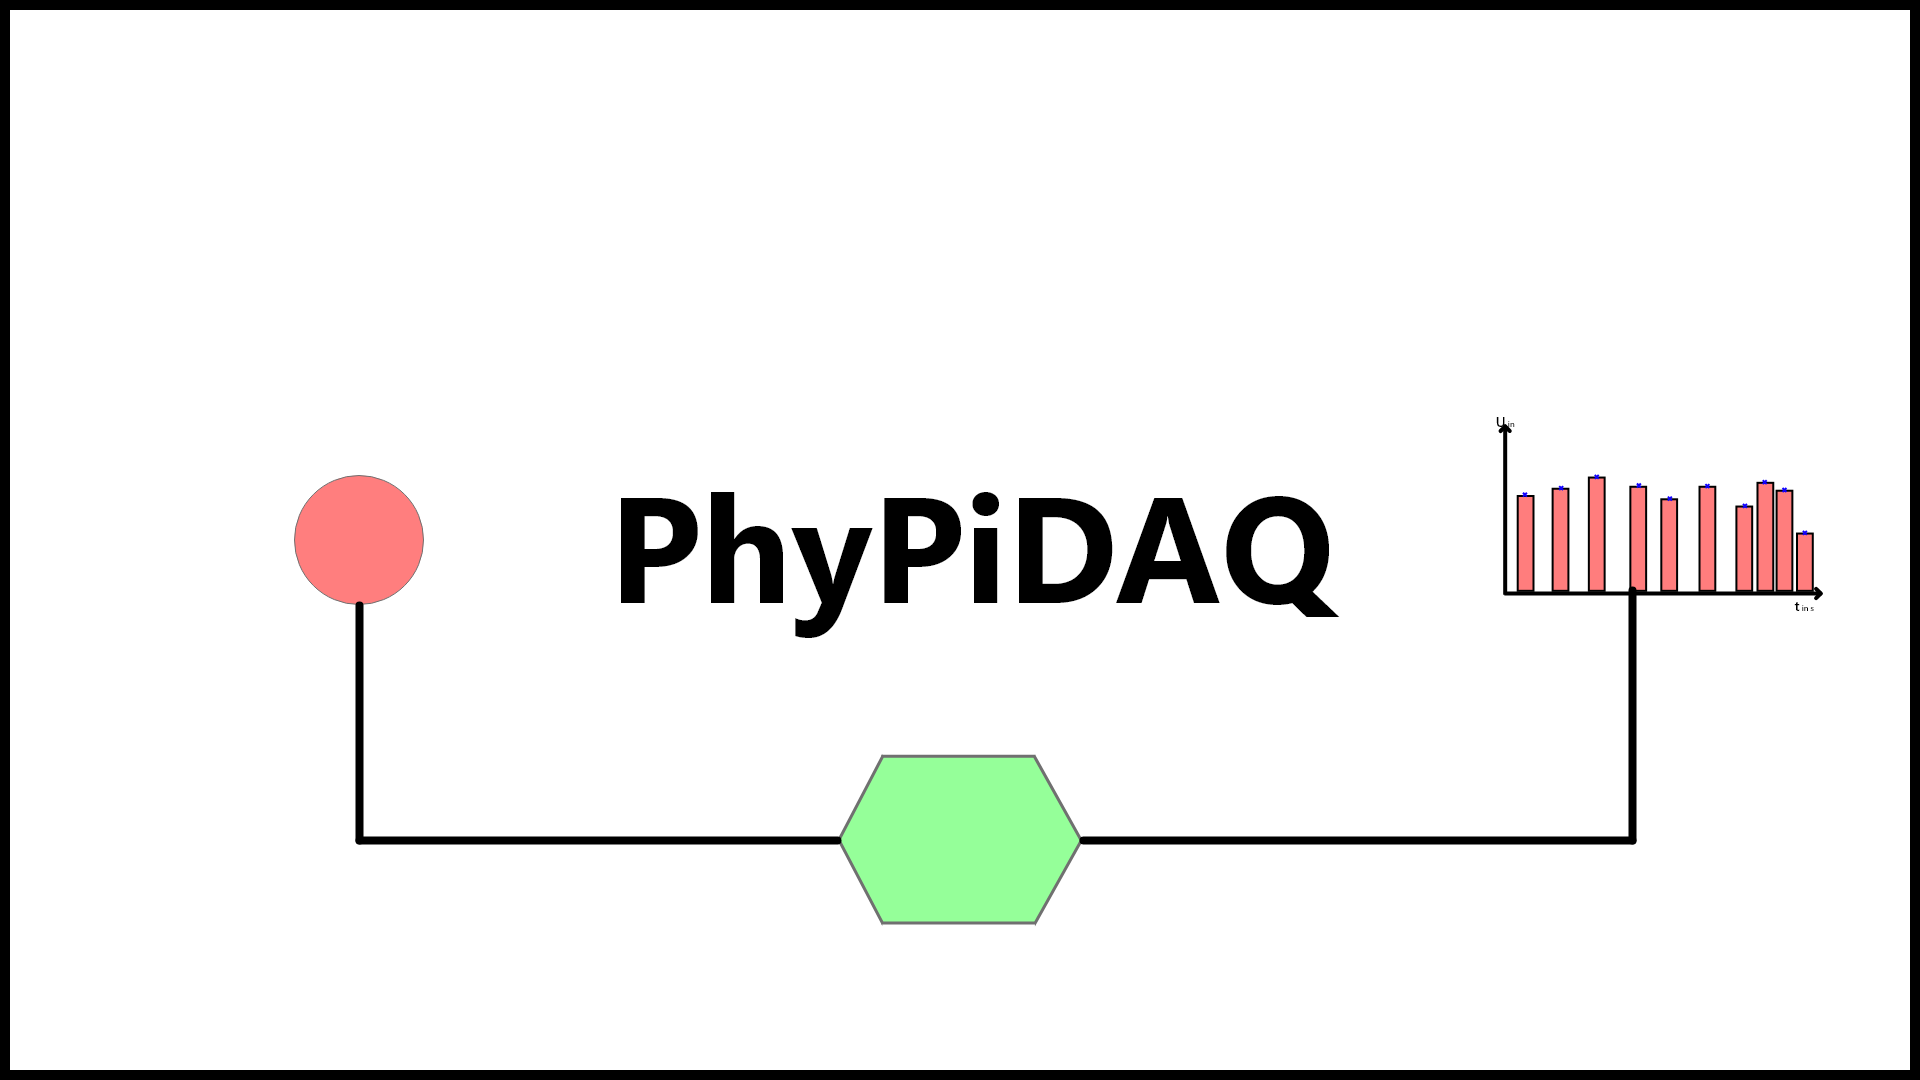
\includegraphics[width = 9cm]{Grafik/Startbildschirm.png}
		\caption{Ein Beispiel für einen Startbildschirm}
		\label{startbildschirm}
	\end{center}
\end{figure}

Eine Erweiterungsmöglichkeit wäre das Einfügen eines Startbildschirmes vor dem Öffnen der Anwendung. Dieser ist in Abbildung \ref{startbildschirm} angedeutet.

\subsubsection{Fehlermeldung}

Für die Fehlermeldungen könnten eigene Fenster erscheinen. Abbildung \ref{fehlerfenster} zeigt ein mögliches Design. Für unterschiedliche Fehler könnten unterschiedliche Designs verwendet werden.

\begin{figure}[htbp]
	\begin{center}
		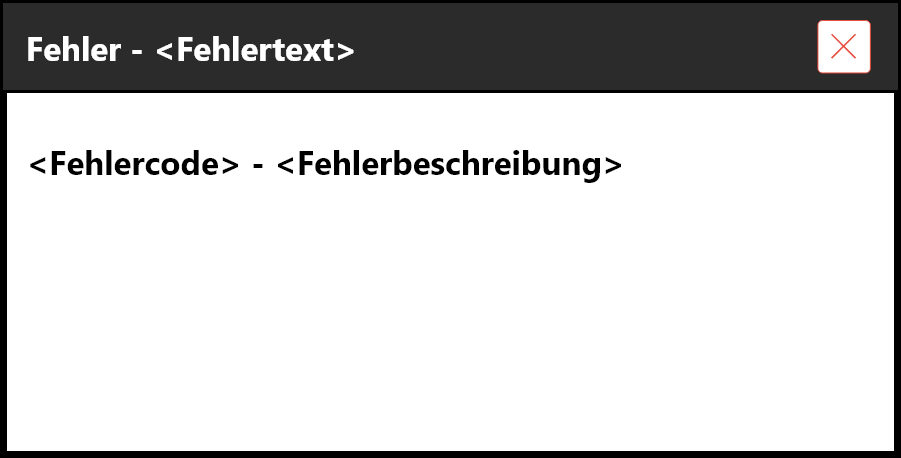
\includegraphics[width = 9cm]{Grafik/Fehlerfenster}
		\caption{Ein Beispiel für ein Fehlermeldungsfenster}
		\label{fehlerfenster}
	\end{center}
\end{figure}

\clearpage
\section{Zeit- und Ressourcenplanung}\label{zeit}

\subsection{Projektphasen}

\begin{tabular}{| l | l | l | r |}
	\hline
	\textbf{Phase} & \textbf{Verantwortlicher} & \textbf{Zeitraum} & \textbf{Kolloquium} \\ \hline
	Pflichtenheft & Jan Küblbeck & KW 20–22 & 04.06.2019 \\
	Entwurf & Leon Huck & KW 23–26 & 02.07.2019 \\
	Implementierung & Stefan Geretschläger & KW 27–29, 31 & 13.08.2019 \\
	Klausurenphase & — & KW 30, 32 & — \\
	Qualitätssicherung & David Gawron & KW 33–35 & 03.09.2019 \\
	Abnahme & — & KW 36 & — \\
	Abschlussprüfung & Linus Ruhnke & KW 37/38 & (tbd) \\
	\hline
\end{tabular}

\subsection{Risikomanagement}

Das Ausfallen eines Teammitglieds durch Krankheit oder anderen Gründen ist ein bedeutendes Risiko. In diesem Fall muss die zusätzliche Arbeit gerecht auf die anderen Teilnehmer verteilt werden. Eventuell können dadurch einzelne Kriterien und Anforderungen nicht mehr zufriedenstellend erfüllt werden.

\subsection{Spezielle Anforderungen}\label{entwicklungsumgebung}

Für die Umsetzung des Projekts ist Zugang zu funktionierender Hardware (konkret: mindestens ein \gls{RasPi}, möglichst mehrere \glspl{sensor}, Peripheriegeräte) notwendig, um die Funktionalität des Produkts sicherzustellen.\newline
Ansonsten muss gegebenenfalls auf simulierte \gls{messdaten} zurückgegriffen werden.

Das Projekt ist von \gls{PhyPiDAQ} abhängig, das heißt Funktionen welche in PhyPiDAQ fehlerhaft sind können möglicherweise nicht korrekt implementiert werden. PhyPiDAQ sollte beispielsweise im Fall eines Programmfehlers eindeutige Fehlercodes produzieren, damit der Benutzer aussagekräftig über das Problem informiert werden kann.

\clearpage
\section{Glossar}\label{glossar}

\renewcommand*{\glossarysection}[2][]{}	% prevents double glossary section heading
\printnoidxglossaries				% generate pdf twice when adding new entries


\end{document}\grid
